\documentclass[reqno,10pt]{amsart}
\usepackage[letterpaper, margin=1in]{geometry}
\RequirePackage{amsmath,amssymb,amsthm,graphicx,mathrsfs,url,slashed,subcaption}
\RequirePackage[usenames,dvipsnames]{xcolor}
\RequirePackage[colorlinks=true,linkcolor=Red,citecolor=Green]{hyperref}
\RequirePackage{amsxtra}
\usepackage{cancel}
\usepackage{tikz-cd}

% \setlength{\textheight}{9.3in} \setlength{\oddsidemargin}{-0.25in}
% \setlength{\evensidemargin}{-0.25in} \setlength{\textwidth}{7in}
% \setlength{\topmargin}{-0.25in} \setlength{\headheight}{0.18in}
% \setlength{\marginparwidth}{1.0in}
% \setlength{\abovedisplayskip}{0.2in}
% \setlength{\belowdisplayskip}{0.2in}
% \setlength{\parskip}{0.05in}
%\renewcommand{\baselinestretch}{1.05}

\title{Functions of least gradient and minimal laminations in constant curvature}
\author{Aidan Backus}
\date{July 2022}

\newcommand{\NN}{\mathbf{N}}
\newcommand{\ZZ}{\mathbf{Z}}
\newcommand{\QQ}{\mathbf{Q}}
\newcommand{\RR}{\mathbf{R}}
\newcommand{\CC}{\mathbf{C}}
\newcommand{\DD}{\mathbf{D}}
\newcommand{\PP}{\mathbf P}
\newcommand{\MM}{\mathbf M}
\newcommand{\II}{\mathbf I}
\newcommand{\Hyp}{\mathbf H}
\newcommand{\Sph}{\mathbf S}
\newcommand{\Group}{\mathbf G}
\newcommand{\GL}{\mathbf{GL}}
\newcommand{\Orth}{\mathbf{O}}
\newcommand{\SpOrth}{\mathbf{SO}}
\newcommand{\Ball}{\mathbf{B}}

\DeclareMathOperator*{\Expect}{\mathbf E}

\DeclareMathOperator{\avg}{avg}
\DeclareMathOperator{\card}{card}
\DeclareMathOperator{\cent}{center}
\DeclareMathOperator{\ch}{ch}
\DeclareMathOperator{\codim}{codim}
\DeclareMathOperator{\Cyl}{Cyl}
\DeclareMathOperator{\diag}{diag}
\DeclareMathOperator{\diam}{diam}
\DeclareMathOperator{\dom}{dom}
\DeclareMathOperator{\Exc}{Exc}
\newcommand{\ext}{\mathrm{ext}}
\DeclareMathOperator{\Gal}{Gal}
\DeclareMathOperator{\Hom}{Hom}
\DeclareMathOperator{\Iso}{Iso}
\DeclareMathOperator{\Jac}{Jac}
\DeclareMathOperator{\Lip}{Lip}
\DeclareMathOperator{\Met}{Met}
\DeclareMathOperator{\id}{id}
\DeclareMathOperator{\rad}{rad}
\DeclareMathOperator{\rank}{rank}
\DeclareMathOperator{\Rm}{Rm}
\DeclareMathOperator{\Hess}{Hess}
\DeclareMathOperator{\Hol}{Hol}
\DeclareMathOperator{\Prop}{Prop}
\DeclareMathOperator{\Radon}{Radon}
\DeclareMathOperator*{\Res}{Res}
\DeclareMathOperator{\sgn}{sgn}
\DeclareMathOperator{\singsupp}{sing~supp}
\DeclareMathOperator{\Spec}{Spec}
\DeclareMathOperator{\supp}{supp}
\DeclareMathOperator{\Tan}{Tan}
\newcommand{\tr}{\operatorname{tr}}

\newcommand{\Mink}{\mathbf m}
\newcommand{\Ric}{\mathrm{Ric}}
\newcommand{\Riem}{\mathrm{Riem}}
\newcommand*\dif{\mathop{}\!\mathrm{d}}
\newcommand*\Dif{\mathop{}\!\mathrm{D}}
\newcommand{\LapQL}{\Delta^{\mathrm{ql}}}

\newcommand{\dbar}{\overline \partial}

\DeclareMathOperator{\atanh}{atanh}
\DeclareMathOperator{\csch}{csch}
\DeclareMathOperator{\sech}{sech}

\DeclareMathOperator{\Div}{div}
\DeclareMathOperator{\Gram}{Gram}
\DeclareMathOperator{\grad}{grad}
\DeclareMathOperator{\dist}{dist}
\DeclareMathOperator{\spn}{span}
\DeclareMathOperator{\Ell}{Ell}
\DeclareMathOperator{\WF}{WF}

\newcommand{\Lagrange}{\mathscr L}
\newcommand{\DirQL}{\mathscr D^{\mathrm{ql}}}
\newcommand{\DirL}{\mathscr D}

\newcommand{\Hilb}{\mathcal H}
\newcommand{\Homology}{\mathrm H}
\newcommand{\normal}{\mathbf n}
\newcommand{\radial}{\mathbf r}
\newcommand{\evect}{\mathbf e}
\newcommand{\vol}{\mathrm{vol}}

\newcommand{\pic}{\vspace{30mm}}
\newcommand{\dfn}[1]{\emph{#1}\index{#1}}

\renewcommand{\Re}{\operatorname{Re}}
\renewcommand{\Im}{\operatorname{Im}}

\newcommand{\loc}{\mathrm{loc}}
\newcommand{\cpt}{\mathrm{cpt}}

\def\Japan#1{\left \langle #1 \right \rangle}

\newtheorem{theorem}{Theorem}[section]
\newtheorem{badtheorem}[theorem]{``Theorem"}
\newtheorem{prop}[theorem]{Proposition}
\newtheorem{lemma}[theorem]{Lemma}
\newtheorem{sublemma}[theorem]{Sublemma}
\newtheorem{claim}[theorem]{Claim}
\newtheorem{proposition}[theorem]{Proposition}
\newtheorem{corollary}[theorem]{Corollary}
\newtheorem{conjecture}[theorem]{Conjecture}
\newtheorem{axiom}[theorem]{Axiom}
\newtheorem{assumption}[theorem]{Assumption}

\theoremstyle{definition}
\newtheorem{definition}[theorem]{Definition}
\newtheorem{remark}[theorem]{Remark}
\newtheorem{example}[theorem]{Example}
\newtheorem{notation}[theorem]{Notation}

\newtheorem{exercise}[theorem]{Discussion topic}
\newtheorem{homework}[theorem]{Homework}
\newtheorem{problem}[theorem]{Problem}

\makeatletter
\newcommand{\proofpart}[2]{%
  \par
  \addvspace{\medskipamount}%
  \noindent\emph{Part #1: #2.}
}
\makeatother

\newtheorem{ack}{Acknowledgements}

\numberwithin{equation}{section}


% Mean
\def\Xint#1{\mathchoice
{\XXint\displaystyle\textstyle{#1}}%
{\XXint\textstyle\scriptstyle{#1}}%
{\XXint\scriptstyle\scriptscriptstyle{#1}}%
{\XXint\scriptscriptstyle\scriptscriptstyle{#1}}%
\!\int}
\def\XXint#1#2#3{{\setbox0=\hbox{$#1{#2#3}{\int}$ }
\vcenter{\hbox{$#2#3$ }}\kern-.6\wd0}}
\def\ddashint{\Xint=}
\def\dashint{\Xint-}

\usepackage[backend=bibtex,style=numeric]{biblatex}
\renewcommand*{\bibfont}{\normalfont\footnotesize}
\addbibresource{topics.bib}
\renewbibmacro{in:}{}
\DeclareFieldFormat{pages}{#1}


\begin{document}
\begin{abstract}
The least-gradient maximum principle, essentially due to Miranda and de Giorgi in the 1960s, shows that least-gradient functions on euclidean space define a minimal lamination of the support of their derivative.
We show that this result holds on manifolds of constant sectional curvature.
As a consequence we answer some questions of Daskalopoulos--Uhlenbeck concerning best-Lipschitz maps, and extend a result of G\'orny about the Radon-Nikod\'ym decomposition of a least-gradient function to the case of constant sectional curvature.
\end{abstract}

\maketitle

%%%%%%%%%%%%%%%%%%%%%%%%%%%%%%%%%%%%%%%%%%%%%%%%%%%%%%%

% \tableofcontents

\section{Introduction}
\subsection{Statement of main results}
Throughout this paper, let $M$ be an oriented Riemannian manifold of metric $g$ and dimension $d$.
For a function $u \in BV_\loc(M)$, we write $\star |\dif u|$ for the total variation of the derivative, c.f. (\ref{total variation}).

\begin{definition}\label{main definitions}
A function $u \in BV_\loc(M)$ has \dfn{least gradient} if for every open $U \Subset M$ and every $v \in BV_\cpt(U)$,
$$\int_U \star |\dif u| \leq \int_U \star |\dif u + \dif v|.$$
A set $U$ of locally finite perimeter has \dfn{least perimeter} if $1_U$ has least gradient.
\end{definition}

Functions of least gradient arise naturally as solutions to an inverse problem in magnetic resonance imaging (MRI) \cite{Nachman2009, Tamasan2019, Joy09} as well as the formal limit of $p$-harmonic functions as $p \to 1$, but we are interested in them primarily because of their application to Thurston's best-Lipschitz maps (see Definition \ref{BestLipDfn}) between closed hyperbolic manifolds \cite{thurston1998minimal}.
An analytic approach to best-Lipschitz maps was introduced by Daskalopoulos--Uhlenbeck \cite{daskalopoulos2020transverse, daskalopoulosPrep1}, where they are viewed as the limit of $p$-harmonic maps as $p \to \infty$, and therefore are ``dual'' in a suitable sense to functions of least gradient.

\subsubsection{The maximum principle}
While we will not need or recall much of Thurston's theory, we recall that a central topic of interest in their study is their interactions with geodesic laminations:

\begin{definition}
A \dfn{minimal lamination} in $M$ is a partition of a closed subset of $M$ into smooth hypersurfaces with zero mean curvature.
If $M$ is a surface we also call $M$ a \dfn{geodesic lamination}.
\end{definition}

The purpose of this paper is to show that functions of least gradient on manifolds $M$ of constant sectional curvature induce minimal laminations in $M$.
This result was already known \cite[Proposition 3.4, Corollary 3.5]{górny2017planar} in the case $M \subseteq \RR^d$, where it was called the \dfn{least-gradient maximum principle}:

\begin{theorem}[maximum principle]\label{main thm}
Let $2 \leq d \leq 7$ and suppose that $M$ has constant sectional curvature.
Let $u \in BV_\loc(M)$, $A_y := \partial \{u > y\}$, $\lambda := \bigcup_{y \in \RR} A_y$.
Then, if $u$ is a function of least gradient:
\begin{enumerate}
\item $\lambda$ is a minimal lamination in $M$,
\item $A_y$ is either empty or a locally finite union of connected hypersurfaces with boundary, and 
\item if $M$ is the interior of a surface-with-boundary $\overline M$, then $\lambda$ extends to a geodesic lamination of $\overline M$.
\end{enumerate}
Conversely, if $\lambda$ is a minimal lamination in $M$, and the set of leaves of $\lambda$ is discrete, then $u$ has least gradient.
\end{theorem}

Theorem \ref{main thm} is called a maximum principle because it implies that if $M$ is the interior of a manifold-with-boundary $\overline M = M \cup \partial M$, then the level sets of any function of least gradient on $M$ must extend all the way to the boundary, just as the maximum principle implies that the level sets of the solution to an elliptic Dirichlet problem should behave.
The existence of $d \leq 7$ is the existence of codimension-$8$ singularities in sets of least perimeter; see \cite[Chapter 11]{Giusti77} for  a discussion of that.

\subsubsection{Applications of the maximum principle}
The maximum principle is a local statement, and we now make precise what it means to be locally a function of least gradient.

\begin{definition}
Let $E \to M$ be an affine line bundle with structure group $\RR$.
A section $u: M \to E$ is \dfn{locally a function of least gradient} valued in $E$ if one can cover $M$ by trivializations $\RR \cong E|U \to U$ of $E$ such that $u|U: U \to E|U$ is a function of least gradient.
\end{definition}

Of particular interest is the case of maps $M \to \Sph^1$, which we may view as sections of a particular affine line bundle whose structure group is $\RR$.
Thus we can speak of \dfn{maps of least gradient} valued in $\Sph^1$.
This will be of especial interest to the applications to hyperbolic and computational geometry, discussed below.

As a consequence of the maximum principle, we show the following analogue of a theorem of G\'orny \cite[Theorem 1.2]{górny2017planar}, which asserts that the Radon-Nikod\'ym decomposition of a map of least gradient has no Cantor part, and that the decomposition preserves the least-gradient condition.

\begin{theorem}[Radon-Nikod\'ym decomposition]\label{Gorny regularity}
Let $2 \leq d \leq 7$ and suppose that $M$ has constant sectional curvature.
Then any map of least gradient $M \to \Sph^1$ can be written as the difference of a continuous section which is locally a function of least gradient, and a section which is locally a function of least gradient and only has jump discontinuities.
\end{theorem}

In the euclidean case, one can also show a well-posedness result \cite[Theorem 1.1]{górny2017planar} using Theorem \ref{Gorny regularity}.
The generalization of this fact is not obvious as we have not extended the Sternberg--Williams--Ziemer theorem \cite{ZiemerWilliamsSternberg1992} to the Riemannian case, so we state it as a conjecture.

\begin{conjecture}
Let $\overline M = M \cup \partial M$ be a compact, strictly convex surface-with-boundary and constant scalar curvature.
Then there exists a solution of the least-gradient Dirichlet problem on $M$ with data in $BV(\partial M)$.
\end{conjecture}

In \S\ref{hyperbolicApps}, we discuss the application of the maximum principle to best-Lipschitz maps.
We also discuss the numerical implementation of the maximum principle in \S\ref{numerics}.

\subsubsection{Regularity of minimal hypersurfaces}
Let us now discuss the main ingredients in the proof of the maximum principle.
The first is a generalization of Miranda's monotonicity formula \cite[Theorem 2.8]{Miranda66}.
This formula is stronger than monotonicity formulae for minimal surfaces in Riemannian manifolds that we are aware of (e.g. \cite[\S7]{MarquesXX}) in that it gives a lower bound on the rate of growth of the monotone quantity.

\begin{theorem}[monotonicity formula]\label{monotonicity prestate}
Let $M$ be a Riemannian manifold and $P \in M$. There exists $A \geq 0$ depending continuously on $P$ such that for every function $u$ of least gradient defined near $P$, every exponential normal coordinate system $(x^\mu)$ based at $P$, and $0 < r_1 < r_2 \lesssim 1$,
\begin{align*}
&\left|\int_{r_1}^{r_2} \partial_r \left[r^{1 - d} \int_{B(P, r)} \dif u \wedge \dif x^1 \wedge \cdots \wedge \dif x^{d - 1}\right] \dif r\right|^2 \\
&\qquad \lesssim \left(1 + (d - 1) \log \frac{r_2}{r_1}\right) \left(r_2^{1 - d}\int_{B(P, r_2)} \star |\dif u| \right)\left(\int_{r_1}^{r_2} \partial_r \left[e^{Ar^2} r^{1 - d} \int_{B(P, r)} \star |\dif u|\right] \dif r\right).
\end{align*}
Moreover, if $M$ is flat or has negative Ricci curvature, then we can take $A = 0$.
\end{theorem}

We will never use the conclusion about the Ricci curvature, and only include it as a curiosity item.

The monotonicity formula appears in a number of places in the proof of Theorem \ref{main lma}, but its main purpose is to generalize Miranda's proof \cite{Miranda66} of de Giorgi's regularity theorem \cite{deGiorgi61} to manifolds; we now state this theorem.

\begin{theorem}[regularity of minimal hypersurfaces]\label{main lma}
Let $2 \leq d \leq 7$ and suppose that $M$ has constant sectional curvature.
Then every set of least perimeter in $M$ is bounded by $C^\infty$ minimal hypersurfaces.
\end{theorem}

We refer the reader to the monograph \cite[Part 1]{Giusti77} for a more detailed, English-language exposition of Miranda's argument.
From Theorem \ref{main lma} and general facts about functions of least gradient that appear in \cite{Miranda67}, the proof of Theorem \ref{main thm} is straightforward, and reviewed in \S\ref{Max Princip}.
We prove the regularity theorem by using the monotonicity formula and a Plateau-type equation adapted to manifolds to deduce a generalization, Proposition \ref{de Giorgi}, of the famous de Giorgi lemma to manifolds.

We end this section by remarking that the assumption on the curvature seems technically convenient, but is probably not essential.

\begin{problem}\label{main conj}
    Remove the assumption on constant sectional curvature from all above theorems.
\end{problem}

%%%%%%%%%%%%%%%%%%%%%%%%%%%%%%%%%%%%%%%%%%%%%%%

\subsection{Applications to hyperbolic geometry}\label{hyperbolicApps}
Let $M$ be a closed hyperbolic surface.
Daskalopoulos--Uhlenbeck \cite{daskalopoulos2020transverse} considered best-Lipschitz maps $M \to \Sph^1$. They identified a particularly important class of such maps, the $\infty$-harmonic maps, which are particularly significant because they induce geodesic laminations of $M$.

\begin{definition}\label{BestLipDfn}
Write $L_f$ for the Lipschitz constant of a map $f: M \to N$.
A \dfn{best-Lipschitz map} $u: M \to N$ is a minimizer of $L_u$ in a given homotopy class.
For such a map we define the \dfn{maximum-stretch locus}
$$\lambda_u := \{x \in M: L(x) = \sup L\}$$
where $L(x)$ denotes the local Lipschitz constant of $u$ at $x$.
If a best-Lipschitz map $u: M \to \Sph^1$ is the weak limit in $L^r$ for $r > d$ of $p$-harmonic maps as $p \to \infty$, we call $u$ \dfn{$\infty$-harmonic}.
\end{definition}

\begin{theorem}\label{infinity harmonic laminations}
Suppose that $M$ is a closed hyperbolic surface and $u: M \to \Sph^1$ is $\infty$-harmonic. Then the maximum-stretch locus $\lambda_u$ is a geodesic lamination in $M$.
\end{theorem}

In \cite[\S5]{daskalopoulos2020transverse}, Daskalopoulos--Uhlenbeck prove Theorem \ref{infinity harmonic laminations} by considering the viscosity solution theory of $\infty$-Laplace equation
\begin{equation}\label{infinity laplace}
    \Hess u(\grad u, \grad u) = 0.
\end{equation}
However, the theory of viscosity solutions of (\ref{infinity laplace}) is still nascent, and Daskalopoulos--Uhlenbeck ask \cite[Problem 9.5]{daskalopoulos2020transverse} for a proof of Theorem \ref{infinity harmonic laminations} that bypasses (\ref{infinity laplace}) altogether.

We give a partial resolution of this problem by proving \cite[Theorem-Conjecture 9.6]{daskalopoulos2020transverse}.
Before we state it, we recall from \cite[\S6]{daskalopoulos2020transverse} that to any $\infty$-harmonic map $u: M \to \Sph^1$, one may associate a map of least gradient $v: M \to \Sph^1$, which we call a \dfn{Daskalopoulos-Uhlenbeck dual} of $u$, such that (among other properties) $\supp \dif v \subseteq \lambda_u$.
The proof that a Daskalopoulos-Uhlenbeck dual exists does not use Theorem \ref{infinity harmonic laminations}.
Since $\supp \dif v$ is a geodesic lamination, we conclude from the maximum principle that:

\begin{corollary}\label{maximum stretch contains lamination}
Let $u$ be an $\infty$-harmonic function on a closed hyperbolic surface $M$.
Then $\lambda_u$ contains a geodesic lamination.
\end{corollary}

Thus to resolve \cite[Problem 9.5]{daskalopoulos2020transverse}, one just needs to show the following conjecture.

\begin{conjecture}\label{two laminations agree}
Every $\infty$-harmonic function $u$ on a closed hyperbolic surface has a Daskalopoulos-Uhlenbeck dual $v$ such that $\supp \dif v = \lambda_u$.
\end{conjecture}

Using the maximum principle one can also show a partial converse to the fact that $\dif v$ endows $\lambda_u$ with the structure of an oriented measured lamination.
For the definitions, see \cite[\S8]{daskalopoulos2020transverse} or \cite{Ruelle75}.
This resolves \cite[Problem 9.7]{daskalopoulos2020transverse}.

\begin{corollary}\label{ruelle sullivan antiderivative}
Let $\lambda$ be an oriented, transversely measured geodesic lamination on a closed hyperbolic surface $M$, and let $\dif v$ be the Ruelle-Sullivan $1$-current induced by $\lambda$.
Then $\dif v$ is the derivative of a map of least gradient on $M$.
\end{corollary}
\begin{proof}
As observed in \cite[\S9]{daskalopoulos2020transverse}, if we lift $\dif v$ to a $1$-current $\dif \tilde v$ on the universal cover $\Hyp^2$, then $\dif \tilde v$ is exact and any antiderivative $\tilde v$ of $\dif \tilde v$ has superlevel sets $\{\tilde v \geq y\}$ which are bounded by geodesics.
Moreover we can choose $\tilde v$ to be $\pi_1(M)$-equivariant.
Since the geodesic flow on $\Hyp^2$ is a hyperbolic dynamical system, the lift $\tilde \lambda$ of the geodesic lamination $\lambda$ to a fundamental domain of $M$ has a discrete set of leaves.
Thus we obtain a map of least gradient on $M$, by Theorem \ref{main thm}.
\end{proof}

We conclude with a teaser for some upcoming work, suggested in private communication and \cite[Problems 9.12--9.13]{daskalopoulos2020transverse} by Daskalopoulos--Uhlenbeck.
Let $M$ be a closed hyperbolic threefold and $f: M \to \Sph^1$ a fibration.
Minimal surfaces in $M$ have been studied intensely since the classical work of Uhlenbeck \cite{Uhlenbeck1983ClosedMS}, and it is particularly of interest to find foliations of $M$ whose leaves are minimal surfaces, and which are compatible with the fibration $f$.
By the maximum principle, it suffices to find a map $v: M \to \Sph^1$ of least gradient, such that $\supp \dif v = M$ and $[v] = [f]$.

We would first need to define a good notion of $p$-Laplacian $\Delta_{k,p}$ for $k$-forms on $M$.
Then, given $p \gg 1$ and $\xi \in H^1(M, \RR)$, we could solve the Neumann problem $\Delta_{1, p} u_p = 0$, $[u_p] = \alpha$.
By generalizing Daskalopoulos-Uhlenbeck duality, we hope to show the existence of a $1$-form $\dif v_q$ which is ``dual" in some sense to the $2$-form $\dif u_p$, where $v_q$ can be viewed as a map $M \to \Sph^1$.
Choosing $\xi$ appropriately we obtain $[v_q] = [f]$, and taking the limit $p \to \infty$, we obtain a map $v: M \to \Sph^1$ of least gradient.
We would then have to show that $\supp \dif v = M$.

%%%%%%%%%%%%%%%%%%%%%%%%%%%%%%%%%%%%%
\subsection{Numerical analysis of minimal laminations}\label{numerics}
The maximum principle, when combined with recent work of Loisel \cite{Loisel20}, also furnishes a large class of minimal laminations in space forms which are inexpensive to numerically compute.

We begin by recalling Loisel's theorem \cite[Theorem 1]{Loisel20} on functions of least gradient.

\begin{definition}
By the \dfn{PL finite element space} associated to a triangulation $\mathcal T$ of a polytope $\overline \Omega \subset \RR^d$ we mean the space of all continuous functions $u: \overline \Omega \to \RR$ whose restrictions $u|T$, $T \in \mathcal T$, are linear.
We equip a PL finite element space with the norm inherited from $W^{1, 1}(\Omega) \subset BV(\Omega)$.
By a \dfn{PL trace} we mean a continuous function $f: \partial \Omega \to \RR$ such that if $T \in \mathcal T$ intersects $\partial \Omega$, then $f|T \cap \partial \Omega$ is linear.
\end{definition} 

Following \cite[\S3.2]{Loisel20}, we identify any PL trace $f$ with its \dfn{discrete harmonic prolongation}, that is, the minimizer $v$ of $\int_\Omega \star |\dif v|^2$ in the PL finite element space subject to $v|\partial \Omega = f$.
Thus $||v||_V \lesssim ||f||_{L^1(\partial \Omega)}$.

\begin{theorem}[Loisel]
Let $\Omega$ be a polytope in $\RR^d$ and let $\mathcal T$ be a triangulation of $\Omega$ with quasiuniformity parameter $\lesssim 1$.
Let $V$ be the PL finite element space associated to $\mathcal T$ and let $f$ be a PL trace.
Let $u \in V$ minimize $\int_\Omega \star |\dif u|$ subject to the constraints $u \in V$, $u|\partial \Omega = f$.
Then the barrier method of \cite[\S2.3]{Loisel20} returns $u$ with runtime $\lesssim |\mathcal T|^{1/2} \log (|\mathcal T|\Japan{||f||_V})$.
\end{theorem}

The same argument shows the above result holds when the Hodge star is not necessarily the euclidean Hodge star.
TODO: Confirm this.

Let $M$ be a closed space form, let $\xi \in H^1(M, \ZZ)$ be a cohomology class, and let $u: M \to \Sph^1$ be a map of least gradient such that $\xi = [\dif u]$.
Then we associate to $\xi$ the minimal lamination induced by $u$.
Note that $u$ may not be unique.

TODO: How are all these things stored in memory?

TODO: The algorithm. Turn $\xi$ into Dirichlet data, compute a tolerance, run Loisel's algorithm, and then use the fact that every leaf runs through the boundary to get the leaves.

\begin{proposition}\label{application to Loisel}
Let $M$ be a closed space form, and let $\xi \in H^1(M, \ZZ)$.
Then Algorithm TODO returns the minimal lamination associated to $\xi$.
Moreover, the runtime is TODO.
\end{proposition}

TODO: Do some numerical experiments, show what minimal laminations in a fundamental polytope in $\Hyp^3$ or $\Sph^3$ look like


%%%%%%%%%%%%%%%%%%%%%%%%%%%%%%%%%%%%%
\subsection{Overview of the paper}
We discuss preliminaries in \S\ref{prelims}: we recall known facts about geometric measure theory on Riemannian manifolds, laminations, functions of least gradient, and the Poincar\'e ball model and stereographic projection on $\Hyp^d$ and $\Sph^d$ respectively.

In \S\ref{MollifierSection} we prove the monotonicity formula, Theorem \ref{monotonicity prestate}, and several consequences that we will use later, including Proposition \ref{mollifier quant}, which allows for the mollification of sets of least perimeter.

The main result of the paper is a de Giorgi-type lemma for sets $U$ of least perimeter in $\Sph^d$ and $\Hyp^d$, which we prove in \S\ref{Plateau section}.
This lemma controls the oscillation of the normal vector to $\partial U$ via an induction on scales.
As in the work of Miranda \cite{Miranda66}, the idea is to reduce to the $C^1$ case, where one can apply elliptic theory to the Plateau equation. In the case of the Poincar\'e ball and the stereographic projection, the Plateau equation behaves so similarly to the euclidean Plateau equation that one can actually apply the known elliptic theory for the Plateau equation.

In \S\ref{GornySec}, we prove the regularity theorem, Theorem \ref{main lma}, from the de Giorgi lemma.
We then deduce the maximum principle, Theorem \ref{main thm}, from the regularity theorem, and as applications of the maximum principle prove Theorems \ref{Gorny regularity} and \ref{application to Loisel}.

%%%%%%%%%%%%%%%%%%%%%%%%%%%%%%%%%%%%%%%%%%%%%%%%

\subsection{Acknowledgements}
I would like to thank Georgios Daskalopoulos for suggesting this project and for many helpful discussions; Karen Uhlenbeck for suggesting the application to hyperbolic threefolds; Trent Lucas for helpful discussions about topology; and Christine Breiner for providing me with the references \cite{Allard72,colding2011course}.


%%%%%%%%%%%%%%%%%%%%%%%%%%%%%%%%%%%%%%%%%%%%%%%%%%
\section{Preliminaries}\label{prelims}
\subsection{Notation and conventions}
For tensor fields we shall use the musical isomorphisms $\sharp, \flat$ and the Einstein convention.
When using the Einstein convention, Greek indices range over $0, 1, \dots$ while Latin indices range over $1, \dots$.
If we have a fixed coordinate system $(x^\mu)$, we sometimes suppress it and write $\partial_\mu := \partial_{x^\mu}$; sometimes we also write $y := x^0$.
The operator $\star$ is the Hodge star, thus $\star 1$ is the Riemannian volume form.
On a submanifold $\Sigma$ of codimension $\geq 1$, $\vol_\Sigma$ denotes the induced volume form and $\star_\Sigma$ denotes the induced Hodge star. We also write $\star_\rho := \star_{B(P, \rho)}$ if $P \in M$ is fixed.
We write $\Japan\xi$ for the Japanese norm $\Japan\xi := \sqrt{1 + |\xi|^2}$
of an element $\xi$ of a normed space.
We write $\int_U \omega \wedge \psi$ for the pairing of a de Rham $\ell$-current $\omega$ with a compactly supported $\ell$-form $\psi$ in an open set $U$.
In particular, we have a Poincar\'e duality map which identifies a $d - \ell$-form $\omega$ with the $\ell$-current $\psi \mapsto \int_U \omega \wedge \psi$.
See \cite{simon1983GMT} for the definition of a de Rham current.
We identify the distributional derivative of a function $u$ with the $d-1$-current
$$\int_U \dif u \wedge \psi = -\int_U u \dif \psi.$$
For a vector field $X$, we write $\star (Xu) := \dif u \wedge \star (X^\flat)$.


%%%%%%%%%%%%%%%%%%%%%%%%%%%%%%%%%%%%%%%%%%%%%%%%%%
\subsection{Riemannian measure theory}
We recall the Riemannian analogue of the main results of \cite[Chapter 1]{Giusti77}.
A function $u$ is in $BV(U)$ iff its derivative $\dif u$ has finite total variation
\begin{equation}\label{total variation}
\int_U \star |\dif u| := \sup_{\substack{||\psi||_{C^0} \leq 1\\\supp \psi \Subset V}} \int_U \dif u \wedge \psi.
\end{equation}
Whether a current has locally finite total variation is independent of the Riemannian metric and so $BV_\loc(M)$ is also independently defined.
By \cite[Theorem 4.14]{simon1983GMT}, for every $u \in BV_\loc(M)$, there exists a $\star |\dif u|$-measurable section $f$ of the cosphere bundle $S'M$ such that for every compactly supported $d-1$-form $\psi$,
\begin{equation}\label{RNy formula}
\int_M \dif u \wedge \psi = \int_M f|\dif u| \wedge \psi.
\end{equation}
The section $f$ of (\ref{RNy formula}) is given pointwise $\star |\dif u|$-almost everywhere, in any local coordinates $(x^\mu)$, by
\begin{equation}\label{Lebesgue point definition}
    f(P) = \left[\lim_{r \to 0} \frac{\int_{B(x, r)} \star \partial_\mu u}{\int_{B(x, r)} \star |\dif u|}\right] ~\dif x^\mu,
\end{equation}
according to the Besicovitch differentiation theorem; here we view $(\dif x^\mu)$ as a basis of $T'_PM$.
Whether the limit $f(P)$ in (\ref{Lebesgue point definition}) exists, or indeed its value as a point of $S'_PM$, denotes not depend on the Riemannian metric or the choice of coordinates.

\begin{definition}
The points $P$ for which the limit (\ref{Lebesgue point definition}) exists and satisfies $|f(P)| = 1$ are called the \dfn{Lebesgue points} of $\dif u$.
\end{definition}

\begin{definition}
Let $U$ be a set of locally finite perimeter, and let $u = 1_U$. Then:
\begin{enumerate}
\item The \dfn{measure-theoretic boundary} $\partial U$ is the set of points whose Lebesgue density with respect to $M$ is $\in (0, 1)$.
\item The set of Lebesgue points of $\dif u$ is the \dfn{reduced boundary} $\partial^* U$.
\item The $\star |\dif u|$-measurable $1$-form $f$ defined by (\ref{Lebesgue point definition}) is the \dfn{conormal $1$-form} $\normal_U$ to $\partial U$.
\end{enumerate}
\end{definition}

Our definition of reduced boundary and conormal $1$-form follows \cite[Definition 3.3]{Giusti77} and is due to \cite{deGiorgi55}.
See \cite{Battista_2021} for an equivalent definition of reduced boundary on Riemannian manifolds, and see \cite[Chapter 6]{Pugh02} for the definition of Lebesgue density.

\begin{proposition}\label{locality of Caccioppoli}
    Let $U$ be a set of locally finite perimeter with conormal $1$-form $\normal$.
    Then:
    \begin{enumerate}
    \item $\partial^* U$ is either empty or $d-1$-dimensional in the Hausdorff sense, and is $d-1$-rectifiable.
    \item $\partial^* U$ is a dense subset of $\partial U$.
    \item If $\normal$ extends to a continuous $1$-form on $\partial U$, then $\partial^* U = \partial U$ is a $C^1$ hypersurface.
    \item If $\partial^* U = \partial U$ is a smooth hypersurface, then $\normal$ is the conormal $1$-form on $\partial U$ as defined in differential topology, and $\star |\dif 1_U|$ is the induced volume form on $\partial U$.
\end{enumerate}
\end{proposition}
\begin{proof}
Most of the assertions of this proposition are diffeomorphism-invariant, so we may assume that $M = \RR^d$ and appeal to \cite[Chapters 2-4]{Giusti77}.
The proof that $\star |\dif 1_U|$ is the induced volume form is identical to \cite[Example 1.4]{Giusti77}.
\end{proof}

\begin{definition}
Let $M$ be a Riemannian manifold, let $U$ be a set of locally finite perimeter, and let $E$ be a Borel set.
The \dfn{perimeter} of $U$ in $E$ is
$$|E \cap \partial^* U| := \int_E \star |\dif 1_U|.$$
\end{definition}

\begin{proposition}[coarea formula]\label{Coarea2}
Let $M$ be a Riemannian manifold and $u \in BV_\loc(M)$. Then for every open set $E$,
\begin{equation}\label{coarea formula}
\int_E \star |\dif u| = \int_{-\infty}^\infty |E \cap \partial \{u > y\}| \dif y.
\end{equation}
\end{proposition}
\begin{proof}
We follow \cite[Theorem 1.23]{Giusti77}, which first proves (\ref{coarea formula}) for $u \in C^\infty(\RR^d)$ using piecewise linear functions.
Such functions are not available for our purposes; instead we note that if $u \in C^\infty(\RR^d)$ and $u$ has no critical points then (\ref{coarea formula}) follows from Fubini's theorem, the fact that $|E \cap \partial \{u > y\}|$ is the surface area of $E \cap \{u = y\}$ (by Proposition \ref{locality of Caccioppoli}), and the change-of-variables formula.
However the left-hand side of (\ref{coarea formula}) is unaffected by critical points of $u$, and the right-hand side of (\ref{coarea formula}) is unaffected by critical values of $u$ by Sard's theorem.
So (\ref{coarea formula}) holds for $u \in C^\infty(\RR^d)$.

The rest of the proof is identical to \cite[Theorem 1.23]{Giusti77}, so we omit the details.
Taking a sequence in $C^\infty(M)$ that converges to $u$ in $L^1_\loc(M)$\footnote{Recall that $C^\infty(M)$ is not dense in $BV_\loc(M)$.}, and applying Fatou's lemma and the semicontinuity of total variation, we conclude the $\geq$ direction of (\ref{coarea formula}).
Moreover, Stokes' theorem gives that for every $d-1$-form $\psi$ such that $||\psi||_{L^\infty} \leq 1$ and $\supp \psi \Subset E$,
$$\int_E u \wedge \dif \psi = \int_{-\infty}^\infty \int_E |\psi| \star |\dif 1_{\partial \{u > y\}}| \dif y \leq \int_{-\infty}^\infty |E \cap \partial \{u > y\}| \dif y.$$
Taking the supremum over $\psi$ we obtain the direction $\leq$ in (\ref{coarea formula}).
\end{proof}

\begin{proposition}[Miranda trace theorem]\label{traces}
Let $U \Subset M$ be an open set with Lipschitz boundary.
For every $u \in BV_\loc(U)$ there exists $v \in L^1_\loc(\partial U)$ such that for every $d-1$-form $\psi$,
\begin{equation}\label{Miranda IBP}
\int_U \dif u \wedge \psi + \int_U u \dif \psi = \int_{\partial U} v\psi.
\end{equation}
Moreover, for almost every $x \in \partial U$,
\begin{equation}\label{convergence of trace}
\int_{U \cap B(x, \varepsilon)} \star |v(x) - u| \ll \varepsilon^d.
\end{equation}
\end{proposition}
\begin{proof}
This follows from a partition-of-unity argument and \cite[Teorema 1]{Miranda67}; we omit the details.
\end{proof}

%%%%%%%%%%%%%%%%%%%%%%%%%%%%%%%%%%%%%%%%%%%%%%%%%%

\subsection{Functions of least gradient}\label{LeastGradientFunctions}
Recall that a function $u \in BV_\loc$ has least gradient iff $u$ is a minimizer of the action $\int_B \star |\dif u|$.
We define
$$\eta(u, U) := \inf_{v \in BV_\cpt(U)} \int_U \star |\dif(u + v)|$$
for $u \in BV_\loc(M)$ and $U \Subset M$, so that $u$ has least gradient iff $\eta(u, U) = \int_U \star |\dif u|$ for every $U$.

Suppose that $u, v \in BV_\loc(M)$ and $U \Subset M$ is bounded by a Lipschitz hypersurface $N$. It is straightforward to generalize \cite[Lemma 5.6]{Giusti77}, thus
\begin{equation}
|\eta(u, U) - \eta(v, U)| \leq ||u - v||_{L^1(N)}. \label{a priori estimate 1}
\end{equation}
In case $v = 0$, we note that by (\ref{convergence of trace}), the trace map is a contraction in $L^\infty$ norm, thus
\begin{equation}
\eta(u, U) \leq ||u||_{L^1(N)} \leq |N| \cdot ||u||_{L^\infty(M)}. \label{a priori estimate 2}
\end{equation}

\begin{definition}
A sequence $(u_n)$ in $BV_\loc(M)$ has \dfn{approximately least gradient} if for every open $U \Subset M$,
$$\limsup_{n \to \infty} \int_U \star |\dif u_n| \leq \liminf_{n \to \infty} \eta(u_n, U) < \infty.$$
\end{definition}

\begin{proposition}[Miranda stability theorem]\label{Miranda convergence}
If a sequence of functions $(u_n)$ has approximately least gradient and $u_n \to u$ in $L^1_\loc(M)$, then $u$ has least gradient, and for every open set $U \Subset M$ with Lipschitz boundary such that $\int_{\partial U} \star |\dif u| = 0$, one has
\begin{equation}\label{convergence in total variation}
\lim_{n \to \infty} \int_U \star |\dif u_n| = \int_U \star |\dif u|.
\end{equation}
\end{proposition}
\begin{proof}
The proof is similar to Teorema 3 and Osservazione 3 in \cite{Miranda67}; we just note the necessary modifications.
Suitable generalizations of Teorema 2 and Osservazione 2 follow from Proposition \ref{traces}.
One needs to add a term of size $o(1)$ to the right-hand side of the inequalities (2.8), (2.9), (2.13), and (2.14); however, in the limit, this term vanishes and so the conclusions (2.15) and (2.16) are unaffected.
\end{proof}

\begin{remark}\label{transversality}
The somewhat unusual condition $\int_{\partial U} \star |\dif u| = 0$ refers to the same Radon measure $\star |\dif u|$ that acts on the open sets of $M$, not on a measure that acts on the relatively open subsets of $\partial U$.
It should be interpreted as a transversality condition: if $u$ is the indicator function of a set $Z$ with $C^\infty$ boundary, then $\int_{\partial U} \star |\dif u| = 0$ if $\partial U$ is transverse to $\partial Z$.
In particular, the notion of convergence in the Miranda stability theorem is weaker than convergence in $BV_\loc(M)$.\footnote{Therefore the Dirichlet problem for functions of least gradient is \underline{ill-posed} in general, as the trace morphism is discontinuous with respect to the topology for this notion of convergence. See \cite{spradlin2013traces} for an explicit counterexample.}
\end{remark}

\begin{corollary}\label{compactness}
Every sequence $(u_n)$ of approximately least gradient converges in $L^1_\loc$ and almost everywhere along a subsequence to a function of least gradient $u$ such that for every open set $U \Subset M$ of Lipschitz boundary such that $\int_{\partial U} \star |\dif u| = 0$, one has (\ref{convergence in total variation}).
\end{corollary}
\begin{proof}
By compactness of the natural map $BV_\loc \to L^1_\loc$, $(u_n)$ has a convergent subsequence in $L^1_\loc$ and almost everywhere.
The conditions on the limit $u$ follow from the Miranda stability theorem.
\end{proof}

\begin{proposition}\label{level sets are minimal}
For every function $u$ of least gradient, the superlevel sets $\{u > y\}$ have least perimeter.
If we instead have a sequence $(u_n)$ of approximately least gradient, then $(\{u_n > y\})$ has approximately least perimeter.
\end{proposition}
\begin{proof}
In the proof of \cite[Theorem 1]{BOMBIERI1969}, we replace the coarea formula (replace \cite[Theorem 1.6]{Miranda66} with Proposition \ref{Coarea2}) and the Miranda stability theorem (replace \cite[Teorema 3]{Miranda67} with Proposition \ref{Miranda convergence}).
\end{proof}

%%%%%%%%%%%%%%%%%%%%%%%%%%%%%%%%%%%%%%%%%%%%%%%%%%
\subsection{Normal coordinates}
Let $(M, g)$ be a Riemannian manifold.
For $(P, V) \in TM$, we call any coordinate system $(x^\mu)_{\mu=0}^{d - 1}$ \dfn{based} at $(P, V)$ if $x^\mu(P) = 0$ and $\partial_0(P) = V$.
We sometimes write $y := x^0$ and use $(x^i)$ to refer to $x^1, \dots, x^{d - 1}$.
TODO: Fix this whole section

We specifically refer to the oriented coordinates arising from the exponential map, $\exp_P: T_PM \to M$, as \dfn{exponential normal coordinates}.
Of course the main technical advantage is that they are \dfn{normal} in the sense that they are oriented and
\begin{equation}\label{expand metric}
g_{\mu\nu} = \delta_{\mu\nu} + O(|x|^2)_{\mu\nu}.
\end{equation}
One can of course add more terms to this expansion, and in fact we will later use the third-order expansion of the $\sqrt{\det g}$ in exponential normal coordinates \cite[Lemma 3.4]{schoen1994lectures}:
\begin{equation}\label{expand volume form}
\sqrt{\det g} = 1 - \frac{1}{3} \Ric_{\mu\nu}(P) x^\mu x^\nu + O(|x|^3).
\end{equation}

There is an annoying technicality with exponential normal coordinates: they are not isothermal.\footnote{Suppose that the exponential map is conformal. By checking on planes in the tangent space we may assume that $d = 2$, and hence that $g$ is locally K\"ahler. But every K\"ahler metric with a holomorphic exponential map is flat \cite{MO68766}.} 
To get around this, we introduce coordinates which are isothermal, but still satisfy the estimate (\ref{expand metric}):

\begin{definition}
We call an oriented coordinate system $(x^\mu)$ \dfn{stereographic normal coordinates} with constant sectional curvature $K \in \RR$ if the metric takes the form 
$$g_{\mu\nu} = \frac{\delta_{\mu\nu}}{(1 + K|x|^2)^2}.$$
\end{definition}

For $K = -1$, the stereographic normal coordinates are a rescaling of the Poincar\'e ball model; for $K = 0$, they are just the usual euclidean metric; and for $K = +1$, they arise from the stereographic projection of the sphere.
So it is clear that we can cover any manifold $(M, g)$ of constant sectional curvature $K$ with its associated stereographic normal coordinates, with any desired basepoint in $TM$.

\begin{remark}\label{rotation invariance}
It is clear that $\SpOrth_d$ acts on each stereographic normal chart by isometries.
Moreover, stereographic normal coordinates based at $P$ are uniquely defined up to this rotation-invariance, since local, oriented, based isometries of $\Sph^d$, $\RR^d$, or $\Hyp^d$ are necessarily rotations.
Sometimes it will be convenient to summarize these facts by saying that the bundle $\mathscr S$ of stereographic normal charts on $M$ is a $\SpOrth_d$-bundle on $M$.
\end{remark} 

Following \cite{Giusti77}, we often use the freedom to choose coordinates to assume that the normal vectors to certain hypersurfaces are approximately vertical.
We make this precise by asserting that the conormal $1$-form, when wedged with the below $d-1$-form, should be close to the volume form:

\begin{definition}
Let $(x^\mu)$ be normal coordinates. The \dfn{vertical $d-1$-form} is
\begin{equation}\label{d1 form}
\psi := \dif x^1 \wedge \dif x^2 \wedge \cdots \wedge \dif x^{d - 1}.
\end{equation}
\end{definition}

\begin{definition}
We call two normal coordinate systems $(x^\mu)$ and $(\tilde x^\mu)$ \dfn{compatible} if:
\begin{enumerate}
\item both $(x^\mu)$ and $(\tilde x^\mu)$ are either exponential normal or stereographic normal, and
\item $\dif \tilde x^0$ is a scalar multiple of $\dif x^0$ at $\tilde P$.
\end{enumerate}
\end{definition}

\begin{lemma}\label{compatible verticals}
Let $(x^\mu), (\tilde x^\mu)$ be compatible normal coordinate systems based at $(P, V)$ and $(\tilde P, \tilde V)$ respectively, let $0 < \rho \lesssim 1$, and $\dist(P, \tilde P) < \rho/2$. Then their respective vertical $d-1$-forms satisfy, in a ball of radius $\rho$ centered at $P$,
$$|\psi - \tilde \psi| \lesssim \rho^2.$$
\end{lemma}
\begin{proof}
We compute the Hodge star 
\begin{align*}
|\psi - \tilde \psi| &= |\star \psi - \star \tilde \psi| \\
&= |\sqrt{\det g} g^{11} \cdots g^{(d-1)(d-1)} \dif x^0 - \sqrt{\det \tilde g} \tilde g^{11} \cdots \tilde g^{(d-1)(d-1)} \dif \tilde x^0| \\
&\leq ||g||_{C^0} (||\dif x^0||_{C^0} \cdot |\sqrt{\det g} - \sqrt{\det \tilde g}| + ||\dif x^0||_{C^0} \sum_{i=1}^{d - 1} |g^{ii} - \tilde g^{ii}| + ||g||_{C^0} \cdot |\dif x^0 - \dif \tilde x^0|).
\end{align*}
Here $||g||_{C^0}$ is the maximum of $\sum_{\mu, \nu} ||g_{\mu\nu}||_{C^0}$ and $||\sqrt{\det g}||_{C^0}$.
From (\ref{expand metric}) the first two terms are $\lesssim \rho^2$.
We now write $\xi := \dif \tilde x^0$ in the coordinate system $(x^\mu)$.
It has length $\sqrt{\tilde g^{00}} = \sqrt{g^{00}} + O(\rho^2)$ and forms an angle $\theta$ with $\dif x^0$ satisfying 
$$\cos \theta = \frac{g^{-1}(\dif x^0, \xi)}{\sqrt{g^{-1}(\dif x^0, \dif x^0) g^{-1}(\xi, \xi)}} = g^{0\mu} \xi_\mu (\tilde g^{00} g^{00})^{-1/2}.$$
By the uniqueness statements in Remark \ref{rotation invariance} and the analogous facts for exponential normal coordinates, for $P$ fixed, $\theta$ is uniquely determined by $\tilde P$ and $x$ and in fact is a smooth function $\theta(\tilde P, x)$.
Moreover, $\theta(P, x) = 0$, so $|\theta| \lesssim \rho$.
It follows from the small-angle approximation that
$$|\cos \theta - 1| \leq 2\theta^2 \lesssim \rho^2$$
and hence $g^{-1}(\dif x^0, \dif \tilde x^0) = 1 + O(\rho^2)$.
Since $g^{-1}(\dif x^0, \dif x^0) = 1 + O(\rho^2)$ and similarly for $g^{-1}(\dif \tilde x^0, \dif \tilde x^0)$, the estimate $|\dif x^0 - \dif \tilde x^0| \lesssim \rho^2$ follows.
\end{proof}

\begin{lemma}\label{convexity of balls}
Let $B \Subset M$ be a ball in a manifold $M$ of constant sectional curvature, and let $P \in M$.
Let $\Psi: V \to \tilde V \subseteq \RR^d$ be a stereographic normal chart based at $P$, such that $B \subseteq V$.
Then $B$ is a convex subset of $\tilde V$.
\end{lemma}
\begin{proof}
The distance function is
$$\dist(Q, R) = \operatorname{arsinh} \sqrt{\delta(Q, R)/2}, ~\delta(Q, R) := \frac{|Q - R|^2}{(1 + K|P - Q|^2)(1 + K|P - R|^2)}.$$
Therefore if $B$ is centered on $Q$, there exists $\delta_* > 0$ such that $\partial B$ is cut out by the equation $\delta(Q, R) = \delta_*$.
This equation can be rewritten
$$|Q - R|^2 + AK|P - R|^2 = A$$
for some $A > 0$, which is the equation of an ellipsoid and bounds a convex set.
\end{proof}

Using (\ref{expand volume form}) for exponential normal coordinates, we study the blowup of $M$ at a point $p$ on the reduced boundary of a set $U$ of least perimeter, giving a generalization of the conjunction of \cite[Theorem 9.3]{Giusti77} and \cite[Theorem 6.2.2]{Simons68}.

\begin{definition}
For a function $u$ on $M$, $P \in M$ we define the \dfn{tangent rescaling} of $u$ at $P$ to be the net of functions $u_t: T_PM \to \RR$, given by
$$u_t(v) = u\left(\exp_P(tv)\right).$$
\end{definition}

\begin{proposition}\label{blowup theorem}
Suppose that $U$ is an open set with least perimeter in $B(P, r)$, $P \in \partial^* U$, and $u = 1_U$.
Furthermore, suppose that $d \leq 7$.
Then the tangent rescaling of $u$ converges as $t \to 0$ along a subsequence (that we also denote $t \to 0$) in $L^1_\loc$ and almost everywhere, to the indicator function $v$ of a half-space $C \subset T_PM$ such that $0 \in \partial C$.
Moreover, for every open set $V \Subset T_PM$ of Lipschitz boundary such that $\partial V$ is transverse to $\partial C$,
$$\lim_{t \to 0} \int_V \star |\dif u_t| = \int_V \star |\dif v|.$$
\end{proposition}
\begin{proof}
We claim that the tangent rescaling $(u_t)$ has approximately least gradient in $T_PM$ (where we give $T_PM$ its euclidean metric). If this true, then by Corollary \ref{compactness}, there exists a set $C$ of least perimeter in $T_PM$, such that the tangent rescaling converges to $v := 1_C$ in the desired sense.
But $T_PM$ is isometric to $\RR^d$, $d \leq 7$, so by the Bernstein--Fleming theorem \cite[Theorem 17.3]{Giusti77}, $\partial C$ is a hyperplane.
The fact that $0 \in \partial C$ follows from the fact that $P \in \partial^* U$.

To prove the claim, write $|\cdot|'$, $\star'$ for the notions taken in the tangent space with its euclidean geometry, and write $U_t$ for the set indicated by $u_t$.
If $V$ is a precompact open subset of $T_PM$, $V_t = \{v \in T_PM: tv \in V\}$, then we have the scale-invariance
\begin{equation}\label{almost blowup scale invariance}
|\partial^* U_t \cap V|' = t^{1 - d}|\partial^* U_1 \cap V_{1/t}|'.
\end{equation}
From (\ref{almost blowup scale invariance}) and the Taylor expansion (\ref{expand volume form}),
$$t^{d - 1} |\partial^* U_t \cap V|' = |\partial^* U_1 \cap V_{1/t}|' \leq e^{O(t^2)} |\partial^* U \cap \exp_P(V_{1/t})|.$$
For every $w \in BV_\cpt(V)$, the least-gradient nature of $u$ gives
$$|\partial^* U \cap \exp_P(V_{1/t})| \leq \int_{(\exp_P)_* V_{1/t}} \star |\dif(u + (\exp_P)_* w_{1/t})| \leq e^{O(t^2)} \int_{V_{1/t}} \star'|\dif(u_1 + w_{1/t})|'.$$
Therefore, after applying (\ref{almost blowup scale invariance}) and (\ref{expand volume form}) again,
$$|\partial^* U_t \cap V|' \leq e^{O(t^2)} t^{1 - d} \int_{V_{1/t}} \star' |\dif (u_1 + w_{1/t})| = e^{O(t^2)} \int_V \star' |\dif (u_t + w)|.$$
Since $V,w$ were arbitrary, we conclude that $(u_t)$ has approximately least gradient.
\end{proof}

%%%%%%%%%%%%%%%%%%%%%%%%%%%%%%%%%%%%%%%%%%%%%%%%%%%
\subsection{The global picture} \label{Global picture}
Suppose that $M$ is a compact space form and let $\tilde M \to M$ be its universal cover.
Then a map $u: M \to \Sph^1$ has least gradient iff its lifts $\tilde u: \Omega \to \RR$, where $\Omega$ is any fundamental domain of $M$, are all functions of least gradient.

Following \cite[\S2]{daskalopoulos2020transverse}, we associate to each map $u: M \to \Sph^1$ a cohomology class $\xi \in H^1(M, \ZZ)$ by letting $\xi$ be the pushforward map in homotopy $u_*: \pi_1(M) \to \pi_1(\Sph^1)$.
This really is a cohomology class because, by the Hurcewiz theorem and the universal property of the abelianization, we have natural isomorphisms
$$\Hom(\pi_1(M), \pi_1(\Sph^1)) = \Hom(\pi_1(M), \ZZ) = \Hom(\pi_1(M)^{\mathrm{ab}}, \ZZ) = \Hom(H_1(M, \ZZ), \ZZ) = H^1(M, \ZZ).$$
In the other direction, for $\xi \in H^1(M, \ZZ)$ we can speak of $\xi$-\dfn{equivariant} functions $\tilde u: \tilde M \to \RR$ on the universal cover: viewing $\xi$ as a map $\pi_1(M) \to \ZZ$, these are the functions $\tilde u$ such that for every $g \in \pi_1(M)$,
$$\tilde u(gx) = \tilde u(x) + (\xi, g).$$
If $\xi$ is the cohomology class associated to a map $u: M \to \Sph^1$, then the $\xi$-equivariant functions are exactly those lifts $\tilde v$ of maps $v: M \to \Sph^1$ with the same homotopy class as $u$.

Using the above construction, we now associate a map of least gradient to each first cohomology class:

\begin{proposition}\label{existence of functions of least gradient}
For every $\xi \in H^1(M, \ZZ)$ there exists a map of least gradient $u: M \to \Sph^1$ such that $[\dif u] = \xi$.
\end{proposition}
\begin{proof}
For each $p > 1$ there exists a $p$-harmonic map $u_p: M \to \Sph^1$ whose associated cohomology class is $\xi$; this follows from a standard existence argument in the calculus of variations.
Then by \cite[Proposition 4.1]{daskalopoulos2020transverse} there exists a subsequence $p \to 1$, a de Rham $1$-current $\psi$, and $\xi$-equivariant function $\tilde u$ so that the Poincar\'e duals of $\dif u_p$ converge to $\psi$ in the weak topology of measures, $\psi$ is Poincar\'e dual to $\xi$, and the Poincar\'e dual of $\dif \tilde u$ is the lift of $\psi$.
In particular, by \cite[Theorem 6.10]{daskalopoulos2020transverse}, $\tilde u$ drops to a map $u$ of least gradient.
\end{proof}

\begin{definition}
Let $u \in BV(M)$. The \dfn{jumpset} of $u$ is the set $J_u$ of $x \in M$ such that there exists $\normal \in T_x'M$ and $u(x-) < u(x+) \in \RR$ such that 
\begin{align*}
\lim_{r \to 0} \dashint_{B(x, r) \cap (\exp_x)_* \{v \in T_xM: (\normal, v) > 0\}} \star |u - u(x+)|  & = 0, \\
\lim_{r \to 0} \dashint_{B(x, r) \cap (\exp_x)_* \{v \in T_xM: (\normal, v) < 0\}} \star |u - u(x-)|  & = 0.
\end{align*}
\end{definition}

\begin{lemma}\label{existence of jump graphs}
Let $u \in BV(M)$ satisfy:
\begin{enumerate}
\item $u$ only has jump discontinuities,
\item the jumpset of $u$ is a lamination $\lambda$ of $M$, and 
\item the traces of $u$ along each leaf $N$ of $\lambda$ are constant on $N$.
\end{enumerate}
Then there exists an affine line bundle $E \to M$, whose structure group is $\RR$, and sections $u_j, u_c \in BV(M, E)$ such that $u = u_c - u_j$, $u_c$ has only Cantorian discontinuities, $u_j$ is locally constant on $M \setminus \lambda$, and on each leaf $N$ of $\lambda$, the traces of $u_j$ along $N$ equal those of $u$.
Moreover, up to isomorphism, $E,u_j,u_c$ are unique.
\end{lemma}
\begin{proof}
This result appears on \cite[pp10--11]{górny2017planar} in case $M$ is a convex subset of $\RR^d$; see also \cite[Remark 3.15]{górny2017planar}.
In general we can cover $M$ with charts which map to convex subsets of $\RR^d$ and exploit the locality and diffeomorphism-invariance of the claimed results.
\end{proof}


%%%%%%%%%%%%%%%%%%%%%%%%%%%%%%%%%%%%%%%%%%%%%%%%%%%
\section{Monotonicity and mollification}\label{MollifierSection}
We have two purposes in this section: to prove Theorem \ref{monotonicity prestate} and to show that we can approximate minimal perimeters by $C^1$, approximately minimal perimeters.
Fix normal coordinates $(x^\mu)$, $\mu = 0, \dots, d - 1$, centered on a point $P \in M$.
We also write $B_r := B(P, r)$.
We use spherical coordinates $(\theta^i)$, $i = 1, \dots, d - 1$, on each sphere $\partial B_r$ which are compatible with $(x^\mu)$ in the sense that $x^0 = f(r) \cos \theta^1$, where $f(r) = r + O_K(r^3)$ if $(x^\mu)$ are stereographic normal with constant curvature $K$, or $f(r) = r$ if $(x^\mu)$ are exponential normal.
This is possible because
\begin{equation}\label{partial Br is a variety}
\partial B_r = \{(x^0)^2 + \cdots + (x^{d - 1})^2 = f(r)^2\}.
\end{equation}
TODO: Introduce the $f$ as notation throughout this section.
We write $\dif \sigma$ for the standard measure on $\Sph^{d - 1}$.

\begin{remark}\label{independence of constants}
Let $K$ be a contractible compact set in $M$.
Then all below implied constants may be chosen independently of the choice of $(x^\mu)$ as long as $P \in K$.
This holds because the space of all exponential normal, or stereographic normal, coordinate systems with basepoint in $K$ is the compact set $K \times \SpOrth_d$, c.f. Remark \ref{rotation invariance}.
\end{remark}

%%%%%%%%%%%%%%%%%%%%%%%%%%%%%%%%%
\subsection{Monotonicity formula}
To prepare for the monotonicity formula, we first generalize an estimate that can be isolated from the proof of \cite[Lemma 5.8]{Giusti77}.

\begin{lemma}\label{monotonicity lemma}
Let $u \in C^1(B_R)$, $0 < r_1 < r_2 < R$, and let
$$E(r) = \int_{B_r} \star |\dif u| - \eta(u, r),$$
so that $E(R) = 0$ iff $u$ has least gradient. Then there exists $A \geq 0$ such that for $R > 0$ small,
\begin{equation}\label{monotonicity lemma eqn}
0 \leq \int_{B_{r_2} \setminus B_{r_1}} \star r^{1 - d}\frac{(\partial_ru)^2}{|\dif u|} \leq 2\int_{r_1}^{r_2} \partial_r \left[e^{Ar^2} r^{1-d}\int_{B_r} \star |\dif u|\right] + \frac{O(E(r))}{r^d} \dif r.
\end{equation}
\end{lemma}
\begin{proof}
We fix $s \in [r_1, r_2]$, introduce a competitor $v(r, \theta) = u(s, \theta)$, and allow $A \geq 0$ to be a constant which may vary from line to line.
From the definition of $\eta$,
\begin{equation}\label{consequence of least gradient monotone}
    \eta(u, s) \leq \int_U \star |\dif v| = \int_0^s \int_{\partial B_r} \star_r |\dif v| \dif r.
\end{equation}
Taylor expanding the volume form and the metric \cite[Lemma 3.4]{schoen1994lectures}, and applying $\partial_r v = 0$, we obtain the existence of $A \geq 0$ such that
\begin{equation}\label{introduce the ricci tensor}
\int_{\partial B_r} \star_r |\dif v| \leq e^{As^2} \frac{\tilde r^{d - 1}}{s^{d - 1}} \int_{\partial B_s} \star_s |\dif v|.\
\end{equation}
Applying (\ref{consequence of least gradient monotone}) and Fubini's theorem,
\begin{align*}
\eta(u, s) &\leq  e^{As^2} \int_0^s \frac{r^{d - 1}}{s^{d - 1}} \dif r \cdot \int_{\partial B_s} \star_s |\dif v| = \frac{s e^{As^2}}{d} \int_{\partial B_s} \star_s |\dif v|\\
&\leq \frac{s e^{As^2}}{d - 1} \int_{\partial B_s} \star_s |\dif v|.
\end{align*}
By Gauss' lemma, $\dif v$ is the orthogonal projection of $\dif u$ onto $T' \partial B_s$, and its orthocomplement is $\partial_r u$. Therefore by Taylor's theorem,
$$\int_{\partial B_s} \star_s |\dif v| \leq \int_{\partial B_s} \star_s |\dif u| \sqrt{1 - \frac{(\partial_r u)^2}{|\dif u|^2}} \leq \int_{\partial B_s} \star_s \left[|\dif u| - \frac{(\partial_r u)^2}{2 |\dif u|}\right]$$
or in other words
\begin{align*}
\int_{\partial B_s} \star_s \frac{(\partial_r u)^2}{2|\dif u|} &\leq \int_{\partial B_s} \star_s |\dif u| - \frac{d - 1}{s} e^{-As^2} \eta(u, s)\\
&\leq \int_{\partial B_s} \star_s |\dif u| - \frac{d - 1}{s} e^{-As^2} \int_{B_s} \star |\dif u| - O(s^{-1}E(s)).
\end{align*}
We moreover have for $\tilde A \geq 0$ that
$$e^{-\tilde As^2} \partial_s \left[e^{\tilde As^2} s^{1 - d} \int_{B_s} \star |\dif u|\right] = \left[2\tilde As^{2 - d} - \frac{d - 1}{s^d}\right]\int_{B_s} \star |\dif u| + s^{1 - d} \int_{\partial B_s} \star_s |\dif u|$$
so if we choose $\tilde A$ so that
$$-\frac{d - 1}{s} e^{-As^2} = 2\tilde As - \frac{d - 1}{s}$$
then
$$s^{1 - d} \int_{\partial B_s} \star_s |\dif u| - (d - 1)\frac{e^{-As^2}}{s^d} \int_{B_s} \star|\dif u| \leq e^{-As^2} \partial_s\left(e^{As^2} s^{1 - d} \int_{B_s} \star|\dif u|\right).$$
We moreover have $e^{-As^2} \leq 1$, so we can now integrate with respect to $\dif s$ to conclude the result.
\end{proof}

\begin{proposition}[monotonicity formula]\label{Monotonicity Formula}\label{sharp monotonicity}
There exists $A \geq 0$ (depending continuously on $P$) such that for every function $u$ in least gradient in $B_R$ where $R$ is small, and every $0 < r < R$,
\begin{equation}\label{weak monotone}
\partial_r e^{Ar^2} r^{1 - d} \int_{B_r} \star|\dif u| \geq 0.
\end{equation}
Stronger,
\begin{align}\label{strong monotone}
&\left|\int_{r_1}^{r_2} \partial_r \left[r^{1 - d}\int_{B_r} \dif u \wedge \psi\right] \dif r\right|^2 \\
&\qquad \lesssim \left(1 + (d - 1)\log\frac{r_2}{r_1}\right)r_2^{1 - d}\int_{B_r} \star |\dif u| \int_{r_1}^{r_2} \partial_r \left[e^{Ar^2} r^{1 - d}\int_{B_r} \star |\dif u|\right] \dif r.
\end{align}
\end{proposition}
\begin{proof}
We first compute $\dif u \wedge \psi = \partial_0 u \dif x$
where $\dif x$ is the natural euclidean volume form on $T_PM$.
Moreover, the radial part of $\partial_0$ is $\cos \theta^1$, and $\iota_{\partial_r} \dif x = r^{d - 1} \dif \sigma$.
Thus by (\ref{partial Br is a variety}),
$$\int_{B_r} \dif u \wedge \psi = r^{d - 1}\int_{\partial B_r} u \cos \theta^1 \dif \sigma(\theta)$$
and hence, since $|\cos \theta^1| \leq 1$,
\begin{align}
\left|\int_{r_1}^{r_2} \partial_r \left[r^{1 - d}\int_{B_r} \dif u \wedge \psi\right] \dif r\right|
&= \left|\int_{\Sph^{d - 1}} (u(r_2, \theta) - u(r_1, \theta)) \cos \theta^1 \dif \sigma(\theta)\right| \\
&\leq \int_{\Sph^{d - 1}} |u(r_2, \theta) - u(r_1, \theta)| \dif \sigma(\theta). \label{monotone dump the metric}
\end{align}
The metric $g$ plays no role in (\ref{monotone dump the metric}), so we may use \cite[Lemma 5.3]{Giusti77} to bound
$$\int_{\Sph^{d - 1}} |u(r_2, \theta) - u(r_1, \theta)| \dif \sigma(\theta) \leq \int_{\Sph^{d - 1}} \int_{r_1}^{r_2} r^{1 - d}|\partial_r u(r, \theta)| \dif r \dif\sigma(\theta).$$
To reintroduce the metric we posit that $R$ is small enough that $\dif r \dif \sigma(\theta) \leq \star 2$.
We therefore have
\begin{equation}\label{monotone before cs}
\int_{\Sph^{d - 1}} \int_{r_1}^{r_2} r^{1 - d}|\partial_r u(r, \theta)| \dif r \dif\sigma(\theta) \leq 2 \int_{B_{r_2} \setminus B_{r_1}} \star r^{1 - d}|\partial_r u|
\end{equation}
and if we apply the Cauchy-Schwarz inequality and approximate $u$ by $C^1$ functions (see \cite[pg68]{Giusti77}), it follows from Lemma \ref{monotonicity lemma} that the right-hand side of (\ref{monotone before cs}) is
$$\lesssim \sqrt{\int_{B_{r_2} \setminus B_{r_1}} \star r^{1 - d} |\dif u|} \sqrt{\int_{r_1}^{r_2} \partial_r \left[e^{Ar^2} r^{1-d}\int_{B_r} \star |\dif u|\right] \dif r}.$$
The monotonicity (\ref{weak monotone}) follows at once. To strengthen it we just need to bound $r^{1 - d} |\dif u|$.
Integrating by parts,
\begin{align*}
\int_{B_{r_2} \setminus B_{r_1}} r^{1 - d} |\dif u| &= \int_{r_1}^{r_2} r^{1 - d} \partial_r \int_{B_r} \star |\dif u| \dif r \\
&\leq r^{1 - d} \int_{B_r} \star |\dif u| + (d - 1) \int_{r_1}^{r_2} r^{-d} \int_{B_r} \star |\dif u| \dif r.
\end{align*}
Using (\ref{weak monotone}) we bound this second integral as
\begin{align*}
\int_{r_1}^{r_2} r^{-d} \int_{B_r} \star |\dif u| \dif r &\leq r^{1 - d} \log \frac{r_2}{r_1} \int_{B_{r_2}} \star |\dif u|. \qedhere
\end{align*}
\end{proof}

\begin{remark}\label{Negative Ricci}
If $g$ has negative Ricci curvature and $(x^\mu)$ are exponential normal, then we can take $A = 0$ in (\ref{introduce the ricci tensor}) and hence in (\ref{strong monotone}), according to (\ref{expand volume form}).
Indeed, we have
$$\frac{\star_r 1}{\star_s 1}(\xi) = \frac{r^{d - 1}}{s^{d - 1}} \frac{1 - r^2 \Ric_{\mu \nu}(0) \xi^\mu \xi^\nu/3 + O(r^3)}{1 - s^2 \Ric_{\mu \nu}(0) \xi^\mu \xi^\nu/3 + O(s^3)}$$
which is $\leq 1$ for $r \leq s \lesssim 1$ and $(\Ric_{\mu\nu})$ negative-definite.
\end{remark}

%%%%%%%%%%%%%%%%%%%%%%%%%%%%%%%%%%%%%%%%%%%%%%%%%%%%%%%
\subsection{The codimension of a minimal perimeter}
We now control the surface area of a minimal perimeter, generalizing \cite[Remark 5.13]{Giusti77}.
This gives a quantitative sense in which a minimal perimeter has codimension $1$.
Write $\Ball^\ell$ for the unit ball in $\RR^\ell$.

\begin{lemma}\label{least perimeter minimal size}
For a set $U$ of least perimeter, if $P \in \partial^* U$ and $d \leq 7$, one has
$$\lim_{r \to 0} r^{1 - d} |\partial^* U \cap B(P, r)| = |\Ball^{d - 1}|.$$
\end{lemma}
\begin{proof}
Choose a sequence of $r \to 0$; then there is a subsequence along which the limit in Proposition \ref{blowup theorem} exists for $u = 1_U$.
With notation as in the proof of Proposition \ref{blowup theorem},
$$r^{1 - d} |\partial^* U \cap B(P, r)| = e^{O(r^2)} r^{1 - d}\int_{B'_r} \star'|\dif u_1|' = e^{O(r^2)} \int_{B'_1} \star'|\dif u_r|'.$$
Then $u_r \to 1_C$ for $C$ a half-space, which in particular is transverse to $B'_1$.
So by the Miranda stability theorem and Remark \ref{transversality},
\begin{align*}
\lim_{r \to 0} e^{O(r^2)} \int_{B'_1} \star'|\dif u_r|' &= \int_{B'_1} \star'|\dif 1_C|' = |\partial C \cap B'_1|' = |\Ball^{d - 1}|. \qedhere
\end{align*}
\end{proof}

\begin{proposition}[surface area estimate]\label{doubling dimension}
If $d \leq 7$ then there exists $A \geq 0$ such that for every set $U$ of least perimeter in a ball $B_r = B(P, r)$, with $P \in \partial^* U$, and $r > 0$ small,
$$|\Ball^{d - 1}|e^{-Ar^2}r^{d - 1} \leq |\partial^*U \cap B_r| \leq |\Sph^{d - 1}|e^{Ar^2} r^{d - 1}.$$
\end{proposition}
\begin{proof}
The upper bound on $|\partial^* U \cap B_r|$ is obtained by using (\ref{a priori estimate 2}) and the fact that the surface area of $\partial B_r$ is $|\Sph^{d - 1}|(1 + O(r^2))r^{d - 1}$ (see e.g. \cite{gray1974volume}).
The lower bound is obtained from Proposition \ref{Monotonicity Formula}, which implies that
$$\lim_{\rho \to 0} e^{-A\rho^2} \rho^{1 - d} |\partial^* U \cap B_\rho| \leq |\partial^* U \cap B_r|.$$
The left-hand side is given by Lemma \ref{least perimeter minimal size}.
\end{proof}

%%%%%%%%%%%%%%%%%%%%%%%%%%%%%%%%%%%%%%%%%%%%%%%%%%%%%%%%%%%%%%%%
\subsection{Mollification of sets of least perimeter}
Our goal for this section is to generalize \cite[Lemma 7.5]{Giusti77}, which reduces the study of sets of least perimeter to that of sets with $C^1$ perimeter.

In this section, the convolution $f * g$ of two functions defined near $P$, or the subtraction $x - y$ of two points near $P$, are meant in the sense of the normal coordinates $(x^\mu)$\footnote{and crucially, \underline{not} in terms of the normal coordinates $(\tilde x^\mu)$ that we introduce in the proof of Lemma \ref{mollifier sublemma}} and the volume form $\dif x := \dif x^0 \wedge \cdots \wedge \dif x^{d - 1}$ obtained from them. Following \cite[Chapter 7]{Giusti77} we define the convolution kernel
$$\chi_\varepsilon(x) = \frac{d + 1}{|\Ball^d|} \varepsilon^{-d}1_{|x| < \varepsilon} \left(1 - \frac{|x|}{\varepsilon}\right)$$
For this section only, we write $u_\varepsilon = u * \chi_\varepsilon$ whenever $u \in BV$ is defined near $P$.

Our first goal is to prove a Riemannian analogue of \cite[Theorem 7.3]{Giusti77}, which estimates $(1_U)_\varepsilon$ for $U$ a set of least perimeter.
The argument there required one to cover $\partial^* U$ by small balls and apply the monotonicity formula in each ball.
To deal with the somewhat large number of parameters involved here, it may helpful to think of the case $\Delta = 1$, in which case we have
$$1 \gg \gamma^q \gg \sigma \gg \gamma \gg \varepsilon \gg \varepsilon \delta > 0.$$

\begin{lemma}[control on $u_\varepsilon$ in each ball]\label{mollifier sublemma}
Let $q < \min(1/8, 1/(4(d - 1)))$.
For every $0 < \Delta, \gamma \lesssim 1$, if we let $\varepsilon = \gamma^4 \Delta$, $\sigma = \gamma^{1/(2(d - 1))} \Delta$, $\delta = \gamma^d$, and let $u$ be the indicator function of a set $U$ of least perimeter such that
\begin{equation}\label{hypothesis on mollifier sublemma}
\int_{B_\Delta} \star(|\psi| \cdot |\dif u| - \dif u \wedge \psi) \leq \Delta^{d - 1} \gamma,
\end{equation}
then on $B_{\Delta - 2\sigma}$, if $Q \in \partial^* U$,
$$(1_{B(Q, 2\delta\varepsilon)}(|\psi| \cdot |\dif u| - \star(\dif u \wedge \psi)))_\varepsilon \ll \gamma^q (1_{B(Q, \delta\varepsilon)} |\dif u|)_\varepsilon.$$
\end{lemma}
\begin{proof}
We first claim that for $r > 0$ so small that $B(Q, 2r) \subseteq B_\varepsilon$,
\begin{equation}\label{bound the kernel}
\sup_{y \in B(Q, 2r)} \chi_\varepsilon(x - y) \lesssim \inf_{y \in B(Q, r)} \chi_\varepsilon(x - y).
\end{equation}
In the euclidean case (with constant equal to $4$) this result can be isolated from the proof of \cite[Theorem 7.3]{Giusti77}.
Otherwise, we can use the smallness of $\varepsilon$ to approximate $g$-balls by euclidean balls.
This suffices to prove (\ref{bound the kernel}), since $\chi_\varepsilon$ is uniformly continuous.

Now let $V := B(Q, 2\delta\varepsilon)$.
Integrating (\ref{bound the kernel}) against $1_V(|\psi| \cdot |\dif u| - \star(\dif u \wedge \psi))$,
\begin{equation}\label{kernel bounded}
(1_V(|\psi| \cdot |\dif u| - \star(\dif u \wedge \psi)))_\varepsilon(x) \lesssim \inf_{y \in B(Q, \delta\varepsilon)} \chi_\varepsilon(x - y) \int_V \star |\psi| \cdot |\dif u| - \dif u \wedge \psi.
\end{equation}
To estimate the right-hand side of (\ref{kernel bounded}) we introduce a new coordinate system $(\tilde x^\mu)$ of normal coordinates centered on $Q$ which are compatible with $(x^\mu)$ in the sense that $\dif \tilde x^0$ is a scalar multiple of $\dif x^0$ at $Q$.
We write $\tilde g$ for the metric written in these new coordinates, and write
$$\tilde \psi := \dif \tilde x^1 \wedge \cdots \wedge \dif \tilde x^{d - 1}.$$
Then by Lemma \ref{compatible verticals},
\begin{equation}
|\tilde \psi - \psi| \lesssim \varepsilon^2. \label{T vs Ttilde}
\end{equation}
In particular,
\begin{equation}\label{split up T Ttilde}
\int_V \star |\psi| \cdot |\dif u| - \dif u \wedge \psi \leq \int_V \star |\psi| \cdot |\dif u| - \dif u \wedge \tilde \psi + O(\varepsilon^2) \int_V \star |\dif u|.
\end{equation}
The error term here is given by Proposition \ref{doubling dimension} and the assumption $\Delta \lesssim 1$ as $\lesssim \gamma^4 \int_{B(Q, \delta\varepsilon)} \star |\dif u|$.
To estimate the dominant term in (\ref{split up T Ttilde}) we assume that $\gamma$ is chosen so small that $\sigma > 2\delta\varepsilon$, so that if we set $W := B(Q, \sigma)$ and apply Proposition \ref{Monotonicity Formula} and (\ref{T vs Ttilde}) to obtain $A \geq 0$ such that
\begin{align*}
(2\delta\varepsilon)^{1 - d} &\int_V \star |\psi| \cdot |\dif u| - \dif u \wedge \psi \\
&\leq \sigma^{1 - d}\int_W \star |\dif u| + (2\delta\varepsilon)^{1 - d} \int_V \star(|\psi| - 1)|\dif u| + 2A\sigma^{3 - d} \int_W \star |\dif u| - (2\delta\varepsilon)^{1 - d}\int_V \dif u \wedge \psi\\
&\leq \sigma^{1 - d}\int_W \star |\dif u| - \dif u \wedge \psi + (2\delta\varepsilon)^{1 - d} \int_V \star(|\psi| - 1)|\dif u| + 2A\sigma^{3 - d} \int_W \star |\dif u| \\
&\qquad + O(\varepsilon^2 \sigma^{1 - d}) \int_W \star |\dif u| + \sigma^{1 - d}\int_W \dif u \wedge \tilde \psi - (2\delta\varepsilon)^{1 - d}\int_V \dif u \wedge \tilde \psi\\
&=: I_1 + I_2 + I_3 + I_4 + I_5 - I_6.
\end{align*}
We apply (\ref{hypothesis on mollifier sublemma}) to bound $I_1 \leq \gamma^{1/2}$, and we use the Taylor expansion of the metric on $V$ to bound $|\psi| - 1 \lesssim \varepsilon^2$ on $B_\varepsilon$.
By Proposition \ref{doubling dimension} and the assumption $\Delta \lesssim 1$, it follows that $I_2 + I_3 + I_4 \lesssim \gamma^{1/(d - 1)}$.

To estimate $I_5 - I_6$, we apply Proposition \ref{sharp monotonicity}:
\begin{align*}
&\sigma^{1 - d} \int_W \dif u \wedge \tilde \psi - (2\delta\varepsilon)^{1 - d} \int_V \dif u \wedge \tilde \psi \\
&\qquad \lesssim \sqrt{1 + (d - 1) \log \frac{\sigma}{2\delta\varepsilon}} \sqrt{\sigma^{1 - d} \int_W \star |\dif u|} \sqrt{\int_{2\delta\varepsilon}^\sigma \partial_r \left[e^{Ar^2} r^{1 - d} \int_{B(Q, r)} \star |\dif u|\right] \dif r}\\
&\qquad =: J_1 J_2 J_3.
\end{align*}
We have $J_1 \lesssim -\log \gamma$, and from Proposition \ref{doubling dimension} we have $J_2 \lesssim 1$.
So, we need to get a gain from $J_3$, which we do as follows:
\begin{align*}
J_3^2 &\leq \sigma^{1 - d} \int_W \star |\dif u| - (2 \delta \varepsilon)^{1 - d} \int_V \star |\dif u| + 2A\sigma^{3 - d} \int_W \star |\dif u| \\
&= \sigma^{1 - d} \int_W \star |\dif u| - \dif u \wedge \psi + \sigma^{1 - d} \int_W \dif u \wedge (\psi - \tilde \psi) + \sigma^{1 - d} \int_W \dif u \wedge \tilde \psi \\
&\qquad - (2 \delta\varepsilon)^{1 - d} \int_V \star |\dif u| + 2A \sigma^{3 - d} \int_W \star |\dif u| \\
&=: K_1 + K_2 + K_3 - K_4 + K_5.
\end{align*}
Then $K_1 = I_1 \leq \gamma^{1/2}$, $K_2 \lesssim I_3 \lesssim \gamma^4$, and $K_5 = I_2 \lesssim \gamma^{1/(d - 1)}$.

To estimate $K_3 - K_4$ we observe that for $u = 1_U$,
\begin{equation}\label{K3 calculus}
K_3 = \sigma^{1 - d} \int_W \dif u \wedge \tilde \psi = \sigma^{1 - d} \int_{U \cap \partial W} \tilde \psi.
\end{equation}
We decompose
$$\partial W = \Gamma_+ \cup \Gamma_0 \cup \Gamma_-$$
where $\tilde x^0 > 0$ on $\Gamma_+$ and $\tilde x^0 < 0$ on $\Gamma_-$. Then all positive contributions to the integral in the right-hand side of (\ref{K3 calculus}) come from $\Gamma_+$.
Moreover, as $d-1$-cells in $M$, $\partial \Gamma_+ = \Gamma_0$, but also if we set $N = \{\tilde x^0 = 0\}$ and $W_0 = W \cap N$, then $\Gamma_0 = \partial W_0$.
In particular, there is a homotopy relating $\Gamma_+$ and $\partial W_0$ which holds $\Gamma_0$ fixed.
Since $\dif \psi = 0$, we can use (\ref{partial Br is a variety}) as follows:
\begin{align*}
K_3 &\leq \sigma^{1 - d} \int_{\Gamma_+} \tilde \psi = \sigma^{1 - d} \int_{W_0} \tilde \psi = |\Ball^{d - 1}|.
\end{align*}
Hence by Proposition \ref{doubling dimension},
$$K_3 \leq |\Ball^{d - 1}| \leq K_4 e^{O(\varepsilon\delta)^2} \leq K_4 + O(\varepsilon\delta)^2 \leq K_4 + O(\gamma^{8 + 2d}).$$
In conclusion, $J_3 \lesssim \gamma^{\min(1/4, 1/(2(d - 1)))}$, and hence by (\ref{kernel bounded}) we have
$$(1_V(|\dif u| - \star(\dif u \wedge \psi)))_\varepsilon(x) \ll (\delta\varepsilon)^{d - 1} \gamma^q \inf_{y \in B(Q, \delta\varepsilon)} \chi_\varepsilon(x - y).$$
Finally, by Proposition \ref{doubling dimension},
\begin{align*}
(\delta\varepsilon)^{d - 1} \inf_{y \in B(Q, \delta\varepsilon)} \chi_\varepsilon(x - y) &\lesssim (1_{B(Q, \delta\varepsilon)} |\dif u|)_\varepsilon(x). \qedhere
\end{align*}
\end{proof}

\begin{lemma}[control on $u_\varepsilon$]\label{main mollifier lemma}
Let $q < \min(1/8, 1/(4(d - 1)))$. There exists $c > 0$ such that for every $0 < \Delta \lesssim 1$ such that for every $0 < \gamma \lesssim 1$ and every indicator function $u$ of a set $U$ of least perimeter such that
\begin{equation}\label{hypothesis on main mollifier lemma}
\int_{B_\Delta} \star |\psi| \cdot |\dif u| - \dif u \wedge \psi \leq \gamma \Delta^{d - 1},
\end{equation}
if we let $\varepsilon = \gamma^4\Delta$, $\sigma = \gamma^{1/(2(d - 1))}\Delta$, and $\varphi = u_\varepsilon$, then on $B_{\Delta - 2\sigma} \cap \{c\gamma^2 < \varphi < 1 - c\gamma^2\}$,
\begin{equation}\label{claim on main mollifier lemma}
(1 - o(\gamma^q)) |\psi| \cdot |\dif \varphi| \leq \star(\dif \varphi \wedge \psi)
\end{equation}
and for every $y \in (c\gamma^2, 1 - c\gamma^2)$,
\begin{equation}\label{claim 2 on main mollifier lemma}
\text{the level set } \partial \{\varphi > y\} \cap B_{\Delta - 2\sigma} \text{ is a }C^1\text{ hypersurface}.
\end{equation}
\end{lemma}
\begin{proof}
Let $\delta = \gamma^d > 0$.
By running a greedy algorithm, we construct a cover $\mathcal V = \{V_n: 1 \leq n \leq N\}$ of $\partial^* U \cap B_{\varepsilon(1 - 2\delta)}$ by balls of radius $2\delta\varepsilon$, centered on points $Q_n \in \partial^* U \cap B_{\varepsilon(1 - \delta)}$, which is \dfn{efficient} in the sense that the dilates $V_n/2 := B(Q_n, \delta\varepsilon)$ are disjoint.
We set $V_0 := B_\varepsilon \setminus B_{\varepsilon(1 - 2\delta)}$.

To bring the $\psi$ inside the convolution we compute
\begin{align*}
(|\psi| \cdot |\dif u|)_\varepsilon
&= \int_{B_\varepsilon} |\psi|(x - y) |\dif u|(x - y) \chi_\varepsilon(y) \dif y \\
&= \int_{B_\varepsilon} |\psi|(x) |\dif u|(x - y) \chi_\varepsilon(y) \dif y + \int_{B_\varepsilon} ||\psi|(x - y) - |\psi|(x)| \cdot |\dif u|(x - y) \chi_\varepsilon(y) \dif y
\end{align*}
and observe that since $\psi$ is continuous, $||\psi|(x - y) - |\psi|(x)| \lesssim \varepsilon \lesssim \gamma^4$.
Since $\dif u$ is supported in $\bigcup_n V_n$, it follows that
\begin{equation}\label{sum over cover}
|\psi| \cdot |\dif \varphi| - \star(\dif \varphi \wedge \psi)
\leq O(\gamma^4) |\dif \varphi| + \sum_{n=0}^N (1_{V_n}(|\psi| \cdot |\dif u| - \star(\dif u \wedge \psi)))_\varepsilon.
\end{equation}

We claim that there exists $c > 0$ such that on $B_\sigma \cap \{c\gamma^2 < \varphi < 1 - c\gamma^2\}$,
\begin{equation}\label{V0 case}
(1_{V_0}(|\psi| \cdot |\dif u| - \star(\dif u \wedge \psi)))_\varepsilon \lesssim \gamma |\dif u|_\varepsilon.
\end{equation}
The proof of (\ref{V0 case}) is essentially given by \cite[pg92]{Giusti77}, so we just sketch it.
For $y \in V_0$, $\chi_\varepsilon(x - y) \lesssim \delta/\varepsilon^d$, so using Proposition \ref{doubling dimension}, one can show
$$\int_{V_0} \chi_\varepsilon(x - y)(|\psi| \cdot |\dif u| - \star(\dif u \wedge \psi))(y) \dif y \lesssim \frac{\gamma^d}{\varepsilon}.$$
Here we used $||\psi||_{L^\infty} \lesssim 1$.
One can use \cite[Lemma 7.1]{Giusti77}, the assumption $c\gamma^2 < \varphi < 1 - c\gamma^2$, and the fact that $g$ is a perturbation of the euclidean metric to obtain
$$\int_{B_\varepsilon} \chi_\varepsilon(x - y) |\dif u|(y) \dif y \gtrsim \frac{\gamma^{d - 1}}{\varepsilon}$$
which then implies (\ref{V0 case}).

Since $\mathcal V$ is efficient, we can sum (\ref{V0 case}) and Lemma \ref{mollifier sublemma} over $n$ in (\ref{sum over cover}) to show that (\ref{claim on main mollifier lemma}) holds.
In particular near $\varphi^{-1}(y) \cap B_{\Delta - 2\sigma}$, where $y \in (c\gamma^2, 1 - c\gamma^2)$, one has $|\dif u| > 0$.
Therefore $u$ is a $C^1$ submersion by \cite[Lemma 7.1]{Giusti77}, thus (\ref{claim 2 on main mollifier lemma}) holds.
\end{proof}

\begin{lemma}[some known inequalities]
Suppose that $u = 1_U$ where $U$ has locally finite perimeter, $w = u_\varepsilon$, and $V = \{w > y\}$ where $y \in (0, 1)$.
Then for any submanifold $\iota: E \to M$ and $0 < \varepsilon \lesssim 1$,
\begin{equation}\label{Giusti125}
x|E \cap (U \Delta V)| \leq \frac{1}{\min(y, 1 - y)} \int_E |w - u| \iota^*(\star 1).
\end{equation}
Moreover, if $0 < \tau \lesssim 1$, then
\begin{align}
\int_{B_\tau} \star |w - u| &\lesssim \varepsilon |B_{\tau + \varepsilon} \cap \partial^* U|, \label{Giusti711}\\
\int_{B_\tau} \star (|\dif w| - |\dif u|) &\lesssim |(B_{\tau + \varepsilon} \setminus B_\tau) \cap \partial^* U|. \label{Giusti712}
\end{align}
\end{lemma}
\begin{proof}
The estimate (\ref{Giusti125}) is a straightforward modification of \cite[Lemma 1.25]{Giusti77}.
The estimates (\ref{Giusti711}, \ref{Giusti712}) follow from \cite[Lemma 7.2]{Giusti77} where we use the fact that for $\tau \lesssim 1$, we can impose normal coordinates in which $\star 1$ is approximately the euclidean volume form.
\end{proof}

We now state our main mollification result.
On first reading, it may help to take $P_n = P$, $(x^\mu_n) = (x^\mu)$, $\omega = \star \dif x^\mu$, and $\Delta_n = 1$.
The proof can be viewed as generalizing \cite[Lemma 7.5]{Giusti77}.

\begin{proposition}\label{mollifier quant}
Let $q < \min(1/8, 1/(4(d - 1)))$.
Let $(P_n)$ be a precompact sequence in $M$ and $0 < \Delta_n \lesssim 1$.
Let $U_n$ be a set of least perimeter in $B_n := B(P_n, \Delta_n)$, $(x^\mu_n)$ be a normal coordinate system at $P_n$, let $\psi^n$ be given by (\ref{d1 form}), and
$$\gamma_n := \Delta_n^{1 - d} \int_{B_n} \star |\psi^n| \cdot |\dif 1_{U_n}| - \dif 1_{U_n} \wedge \psi^n.$$
If $(\gamma_n) \in \ell^1$ then for almost every $t \in (0, 1)$ and every $n \in \NN$ there exists a set $V_n$ with $C^1$ boundary in $tB_n := B(P_n, t\Delta_n)$ such that for $n \gg 1$,
\begin{align}
|\partial V_n \cap tB_n| &\leq \eta(V_n, t\Delta_n) + o(\gamma_n \Delta_n^{d - 1}), \label{mollifier quant1}\\
||\partial^* U_n \cap tB_n| - |\partial V_n \cap tB_n|| &\ll \gamma_n \Delta_n^{d - 1}, \label{mollifier quant2}
\end{align}
on $B(P_n, t(1 - 2\sigma_n)\Delta_n)$, where $\sigma_n := \gamma_n^{1/(2(d - 1))}$, one has
\begin{equation}
\star(\normal_{V_n} \wedge \psi^n) \geq |\psi^n| \cdot (1 - o(\gamma^q)), \label{mollifier quant4}
\end{equation}
and for every $d-1$-form $\omega_n$ defined near $P_n$,
\begin{equation}\label{mollifier quant3}
\left|\int_{tB_n} \dif(1_{U_n} - 1_{V_n}) \wedge \omega_n\right| \ll \gamma_n \Delta_n^{d - 1} ||\omega_n||_{C^1}.
\end{equation}
\end{proposition}
\begin{proof}
In this proof, we shall assume that the constants furnished by the above results are uniform in $n$; this is possible by Remark \ref{independence of constants} and the compactness of $\overline{\{P_n: n \in \NN\}}$.

\proofpart{1}{Construction of $V_n$ and proof of (\ref{mollifier quant4})}
Draw $t$ uniformly at random, let $w_n := (u_n)_{\Delta_n \gamma_n^4}$, let $c, q$ be as in Lemma \ref{main mollifier lemma}, and let $a_n = c\gamma_n^2$, $b_n = 1 - c\gamma_n^2$.
By the coarea formula, Proposition \ref{Coarea2},
$$\int_{tB_n} \star |\dif w_n| = \int_0^1 |\partial^* \{w_n > y\} \cap tB_n| \dif y \geq \int_{a_n}^{b_n} |\partial^* \{w_n > y\} \cap tB_n| \dif y,$$
so by the mean value theorem, there exists $y_n \in (a_n, b_n)$ such that
$$|\partial^* \{w_n > y_n\} \cap tB_n| \leq \frac{1}{b_n - a_n} \int_{tB_n} \star |\dif w_n|.$$
We then set $V_n := \{w_n > y_n\}$, $v_n := 1_{V_n}$, so $V_n$ has $C^1$ boundary in $tB_n$ by (\ref{claim 2 on main mollifier lemma}), and by the above computation,
\begin{equation}\label{MVT mollifier}
|V_n \cap tB_n| \leq \frac{1}{1 - 2c\gamma_n^2} \int_{tB_n} \star |\dif w_n|.
\end{equation}
Since $\grad w_n$ is normal to the level sets of $w_n$, $\normal_{V_n} = \dif w_n/|\dif w_n|$.
Hence (\ref{mollifier quant4}) is a consequence of (\ref{claim on main mollifier lemma}).

\proofpart{2}{Auxiliary estimates}
Let $\Gamma_n := \partial(tB_n)$; we claim that almost surely,
\begin{align}
||u_n - v_n||_{L^1(\Gamma_n)} &\ll \Delta_n^{d - 1} \gamma_n \label{trace of vn} \\
|\partial V_n \cap tB_n| &\leq |\partial^* U_n \cap tB_n| + o(\Delta_n^{d - 1} \gamma_n). \label{difference of surface area}
\end{align}
To establish the claim, observe that by (\ref{Giusti711}) and Proposition \ref{doubling dimension},
$$\limsup_{n \to \infty} \Delta_n^{1 - d} \gamma_n^{-4} \int_{tB_n} \star |u_n - w_n| \lesssim \limsup_{n \to \infty} \Delta_n^{2-d} |\partial^* U_n \cap tB_n| \lesssim \sup_n \Delta_n \lesssim 1.$$
Differentiating in $t$, we see that
$$||u_n - w_n||_{L^1(\Gamma_n)} \ll \Delta_n^{d - 1} \gamma_n^3$$
almost surely. So by (\ref{Giusti125}),
$$||u_n - v_n||_{L^1(\Gamma_n)} \lesssim \gamma_n^{-2} ||u_n - w_n||_{L^1(\Gamma_n)} \ll \Delta_n^{d - 1} \gamma_n$$
almost surely, proving (\ref{trace of vn}).
Now let
$$f(s) = \sum_{n=1}^\infty \gamma_n \Delta_n^{1 - d} \int_{sB_n} \star |\dif u_n|.$$
Then $f' \geq 0$, and by Proposition \ref{doubling dimension}, $f(1) \lesssim \sum_n \gamma_n < \infty$.
So almost surely,
$$f(t + \gamma_n^4) - f(t) \lesssim \gamma_n^4$$
and hence
$$\int_{(t + \gamma_n^4)B_n \setminus tB_n} \star |\dif u_n| \lesssim \gamma_n^3 \Delta_n^{d - 1}.$$
From (\ref{Giusti712}) it follows that
$$\int_{tB_n} \star |\dif w_n| \leq \int_{tB_n} \star |\dif u_n| + o(\gamma_n^2).$$
By (\ref{MVT mollifier}) we conclude that (\ref{difference of surface area}) holds almost surely.

\proofpart{3}{Proof of (\ref{mollifier quant1}) and (\ref{mollifier quant2})}
The estimate (\ref{mollifier quant2}) is the conjunction of (\ref{trace of vn}), (\ref{difference of surface area}), and (\ref{a priori estimate 1});
(\ref{mollifier quant1}) is the conjunction of (\ref{mollifier quant2}), (\ref{a priori estimate 1}), the fact that $U_n$ has least perimeter, and (\ref{trace of vn}).

\proofpart{4}{Proof of (\ref{mollifier quant3})}
Integrating by parts,
$$\left|\int_{tB_n} \dif (u_n - v_n) \wedge \omega_n\right| \leq ||\omega_n||_{L^\infty} ||u_n - v_n||_{L^1(\Gamma_n)} + ||\dif \omega_n||_{L^\infty} \int_0^t ||u_n - v_n||_{L^1(\partial(sB_n))} \dif s.$$
By (\ref{trace of vn}),
$$\limsup_{n \to \infty} ||\omega_n||_{C^1}^{-1} \gamma_n^{-1} \Delta_n^{1 - d} \left|\int_{tB_n} \dif(u_n - v_n) \wedge \omega_n\right| \leq \limsup_{n \to \infty} \int_0^t \gamma_n^{-1} \Delta_n^{1 - d} ||u_n - v_n||_{L^1(\partial(sB_n))} \dif s.$$
Moreover, (\ref{trace of vn}) holds with $t$ replaced by almost any $s$, so
$$f_n(s) := \gamma_n^{-1} \Delta_n^{1 - d} ||u_n - v_n||_{L^1(\partial(sB_n))}$$
satisfies $(f_n) \in \ell^\infty([0, 1] \to L^\infty)$, and $f_n \to 0$ almost everywhere.
So by Fatou's lemma,
\begin{align*}
0 \leq \limsup_{n \to \infty} ||\omega_n||_{C^1}^{-1} \gamma_n^{-1} \Delta_n^{1 - d} \left|\int_{tB_n} \dif(u_n - v_n) \wedge \omega_n\right| &\leq \int_0^t \lim_{n \to \infty} f_n(s) \dif s = 0. \qedhere
\end{align*}
\end{proof}


%%%%%%%%%%%%%%%%%%%%%%%%%%%%%%%%%%%%%%%%%%%%%%
\section{de Giorgi lemma}\label{Plateau section}
The main technical result of this section, and indeed of this paper, is a de Giorgi-type lemma, Proposition \ref{de Giorgi}.
Such a lemma is the inductive case of an induction-on-scale argument which ensures that at fine scales, one has control on the conormal $1$-form $\normal_U$ to a set of least perimeter.
Such a result is due to de Giorgi \cite{deGiorgi61}. Miranda \cite{Miranda64, Miranda66} showed that the de Giorgi lemma can be proven using functions of least gradient.
We shall follow Miranda's argument, showing that each stage can be extended to the case of constant sectional curvature without incurring losses that are at all significant.

Given a set $U$ of least perimeter at scale $\rho \ll 1$, the proof proceeds by replacing $U$ with an approximation $V$ with $C^1$ perimeter using the monotonicity formula for least gradient that we proved in the previous section.
We then change coordinates so that $\partial V$ can be represented as the graph of a function $w$ which is small in $C^1$.
We then estimate $w$ in terms of its behavior at scale $2\rho$ using the elliptic theory for the Plateau equation, picking up an error term of size $\rho^d$ when we do so.
By induction, we estimate the behavior of $U$ at scale $\rho$ in terms of its behavior at scale $1$, and the total error terms turn out to be logarithmically small.

Such an argument already appears in \cite{Miranda66}, but with a sequence of ``candidate counterexamples'' $U_n$, no additive error terms, and somewhat fewer changes of coordinates.
We found it convenient to avoid the sequence $(U_n)$, only working with it in technical lemmata where one is forced to appeal to a comapctness argument.
This will be especially convenient for us, as it makes it somewhat easier to juggle the additive errors and coordinate changes.

We fix some constants that we will use throughout this section.
Fix an underlying manifold $(M, g)$ of constant sectional curvature $K \in \RR$.
Fix $0 < \alpha < 1$, $0 < c_0 = c_0(d) \lesssim 1$ to be chosen much later, which depend only on $d := \dim M$.\footnote{These constants are smallest when $d = 7$, namely $c_0 \approx 7.8 \cdot 10^{-4}$, and $\alpha \approx 0.5 + 3.9 \cdot 10^{-4}$. So the reader may take $c_0 := 10^{-3}$, $\alpha := 0.5$ for concreteness.} 
We denote by $c_1, \dots, c_3$ constants with dependence
$$c_i = c_i(d, K, \alpha, c_0, \dots, c_{i - 1}) > 0.$$
These constants arise every time we need to use a compactness argument, so they are ineffective and one expects $c_i \ll c_{i - 1}$.
We let $C > 0$ be a large constant which varies from line to line, but require that $C$ only depends on the $c_i$s that have already been chosen, $d$, and $K$.

%%%%%%%%%%%%%%%%%%%%%%%%%%%%%%

\subsection{Nonparametric minimal hypersurfaces in \texorpdfstring{$\RR^d$}{Rd}}
Let us recall some facts about the Plateau equation for minimal hypersurfaces in $\RR^d$ that we will need later.
We begin by recalling the Weinstein--Aronsazjn formula: for $v, w \in \RR^m$ and $A \in \GL_m$,
\begin{equation}\label{Weinstein Aronsazjn}
\det(A + v \otimes w) = (1 + v \cdot A^{-1}w) \det A.
\end{equation}
We also remind the reader that $\Japan\xi$ denotes the Japanese norm $\sqrt{1 + |\xi|^2}$.

If $v$ is a function on $\RR^{d - 1}$, then we can use diffeomorphism $x \mapsto (x, v(x))$ to impose coordinates on the graph $N$ of $v$; in these coordinates the metric tensor on $N$ can be easily seen to be $1 + \dif v \otimes \dif v$.
Then by (\ref{Weinstein Aronsazjn}), the surface area of $N$ in $\Omega \times \RR$ is $\int_\Omega \Japan{\dif v} \dif x$.
Taking $\Japan{\dif v} \dif x$ as a Lagrangian, we obtain the PDE
\begin{equation}\label{Euclidean Plateau}
\dif^* \left[\frac{\dif v}{\Japan{\dif v}}\right] = 0.
\end{equation}
This equation is the \dfn{Plateau equation} or \dfn{minimal surface equation}.

Following the terminology in \cite{Giusti77}, we make a distinction between \dfn{parametric} minimal hypersurfaces -- that is, boundaries of sets of least perimeter -- and \dfn{nonparametric} minimal hypersurfaces -- that is, the graphs of classical solutions of the Plateau equation -- but we note carefully that the notion of nonparametric surface is not diffeomorphism-invariant.

To third order for $\dif v$ small, the Lagrangian is $1 + |\dif v|^2/2$, whose Euler-Lagrange equation is the Laplace equation $\Delta v = 0$.
That is, (\ref{Euclidean Plateau}) is second-order quasilinear elliptic, and so enjoys elliptic regularity \cite{morrey2009multiple}: if $v$ is a \dfn{variational solution} in the sense that it is a $H^1_\loc$ minimizer\footnote{In practice, we will only need to consider Lipschitz minimizers, which are clearly $H^1_\loc$.} of the Lagrangian, then $v$ is actually a \dfn{classical solution} in the sense that it is a $C^\infty$ solution of (\ref{Euclidean Plateau}).

The PDE (\ref{Euclidean Plateau}) enjoys scaling-invariance.
More precisely, if we set
\begin{equation}\label{rescaled solution}
v_\lambda(x) := v(\lambda x)/\lambda,
\end{equation}
then $\dif v_\lambda(x) = (\dif v)(\lambda x)$ and hence the Lagrangian is scale-invariant:
\begin{equation}\label{Lagrange is scale invariant}
\Japan{\dif v_\lambda(x)} = \Japan{\dif v(\lambda x)}.
\end{equation}
In particular, (\ref{Euclidean Plateau}) is preserved by the scaling (\ref{rescaled solution}).
Of course, the linearized operator $\Delta$ is also preserved by (\ref{rescaled solution}).

We define for a $1$-form $\xi: \RR^{d - 1} \to (\RR^{d - 1})'$ and $\rho > 0$, the $1$-form $\avg_\rho \xi$ which acts on vectors $v \in T_x\RR^{d - 1} = \RR^{d - 1}$ by
\begin{equation}\label{definition of averaging}
(\avg_\rho \xi(x), v) := \dashint_{B_\rho} (\xi(x), v) \dif x
\end{equation}
where $B_\rho \subset \RR^{d - 1}$.\footnote{Beware: (\ref{definition of averaging}) relies on the flatness of the Levi-Civita connection to make the identifications $T_x\RR^{d - 1} = \RR^{d - 1}$ and $T'\RR^{d - 1} = \RR^{d - 1} \times (\RR^{d - 1})'$, so that we \underline{cannot} replace $\RR^{d - 1}$ with a curved space in this definition.}

Using the mean-value property of the linearized Plateau operator $\Delta$, de Giorgi \cite{deGiorgi61} proved the following key estimate on approximate variational solutions of the Plateau equation. As we have not succeeded in obtaining a copy of \cite{deGiorgi61} we refer the reader to \cite{Miranda66} for the proof.

\begin{lemma}[de Giorgi lemma, euclidean Plateau case]\label{Miranda42 quant}
There exists $c_1 = c_1(d, c_0) > 0$ such that the following holds.
Let $\beta, \rho > 0$, $0 < \alpha' < 1$, $w \in C^1(B_\rho)$, and let $u$ be the harmonic function on $B_\rho$ with $u|\partial B_\rho = w|\partial B_\rho$.
If $||\dif w||_{C^0} \leq c_1$,
\begin{align}
\int_{B_\rho} \Japan{\dif w} - \Japan{\avg_\rho \dif w} \dif x &\leq \beta, \label{Miranda42 hyp} \\
\int_{B_\rho} \Japan{\dif w} - \Japan{\dif u} \dif x &\leq c_1 \beta,
\end{align}
then 
\begin{equation}\label{Miranda42 concl}
\int_{B_{\alpha' \rho}} \Japan{\dif w} - \Japan{\avg_{\alpha' \rho} \dif w} \dif x \leq ((\alpha')^{d + 1} + c_0) \beta.
\end{equation}
\end{lemma}
\begin{proof}
If not, then there exist tuples $(w_n, u_n, \rho_n, \beta_n)$ such that $||\dif w_n||_{C^0(B_{\rho_n})} \leq 1/n$,
$$\int_{B_{\rho_n}} \Japan{\dif w_n} - \Japan{\dif u_n} \dif x \leq \frac{\beta_n}{n},$$
and (\ref{Miranda42 hyp}) holds, but (\ref{Miranda42 concl}) fails. 
Using the rescaling (\ref{rescaled solution}), we may assume that $\rho_n$ is some fixed $\rho$; then for $n$ large this contradicts \cite[Lemma 4.2]{Miranda66}. 
\end{proof}

\subsection{Nonparametric minimal hypersurfaces in \texorpdfstring{$M$}{M}}
We now derive a Plateau-type equation for manifolds.

\begin{lemma}\label{Plateau setup lemma}
Let $(x^i, y)$ be stereographic normal coordinates.
Let $w \in C^1(\Omega)$, $\Omega \subseteq \RR^{d - 1}$.
Parametrize
\begin{equation}\label{definition of graph}
N_w := \{(x, w(x)) \in M: x \in \Omega\}
\end{equation}
using the $C^1$-diffeomorphism $\Psi_w(x) = (x, w(x))$. Then there exists $F \in C^\infty(\Omega \times \RR)$ such that $F(0, 0) = 1$, $\dif F(0, 0) = 0$, and:
\begin{enumerate}
\item The restriction of $g$ to $N_w$ pulls back as
\begin{equation}\label{restricted metric in isothermal coords}
\Psi_w^*(g|N_w) = F(x, w(x))^{\frac{2}{d - 1}}(\dif x^2 + \dif w^2).
\end{equation}
\item The induced volume form on $N_w$ pulls back as
\begin{equation}\label{restricted measure in isothermal coords}
\Psi_w^*(\iota_{\normal_{N_w}}(\star 1)) = F(x, w(x)) \Japan{\dif w(x)} \dif x
\end{equation}
where $|\cdot|$ is the standard metric on $\RR^{d - 1}$.
\item The upwards conormal $1$-form is
\begin{equation}\label{conormal in isothermal coords}
\normal_U(x, w(x)) = F(x, w(x))^{\frac{1}{d - 1}} \frac{\dif y - \partial_i w(x) \dif x^i}{\Japan{\dif w(x)}}.
\end{equation}
\end{enumerate}
\end{lemma}
\begin{proof}
Let $(\partial_i)$ be the standard frame on $\Omega$.
Then 
$$\dif \Psi_w = \begin{bmatrix}I \\ \dif w\end{bmatrix}$$
so
$$g(\dif \Psi_w \cdot \partial_i, \dif \Psi_w \cdot \partial_j) = (1 + O(|x|^2) + O(w(x)^2))(\dif x^2(\partial_i, \partial_j) + \partial_i w \partial_j w)$$
and hence (\ref{restricted metric in isothermal coords}) holds.
Moreover, by the Weinstein--Aronsazjn theorem (\ref{Weinstein Aronsazjn}),
\begin{align*}
\sqrt{\det(\dif x^2 + \dif w^2)} &= \sqrt{\det(1 + \dif w \otimes \dif w)} \dif x = \sqrt{1 + |\dif w|^2} \dif x
\end{align*}
wheich proves (\ref{restricted measure in isothermal coords}).
Finally, we observe that if $F = 1$ (thus $g$ is flat) then 
\begin{equation}\label{conormal on flat space}
\normal_U(x, w(x)) = \frac{\dif y - \partial_i w(x) \dif x^i}{\sqrt{1 + |\dif w|^2}},
\end{equation}
and since $(x^\mu)$ are isothermal, in the general case $\normal_U$ must be the $1$-form in (\ref{conormal on flat space}) multiplied by a scalar field to have unit length.
This proves (\ref{conormal in isothermal coords}).
\end{proof}

\begin{definition}
For a fixed choice $(x, y)$ of stereographic normal coordinates, define the Lagrangian
$$\Lagrange(y, \xi) := F(x, y) \Japan{\xi} \dif x.$$
Let $w \in H^1_\loc(\Omega)$, and let $N_w, \Psi_w$ be given by (\ref{definition of graph}).
The \dfn{Plateau energy} of $w$ is $\Lagrange(w, \dif w)$.
The \dfn{Plateau equation} is the Euler-Lagrange equation for the Plateau energy.
\end{definition}

\begin{lemma}\label{Plateau wellposedness}
The Plateau equation is
\begin{equation}\label{Plateau eqn}
\dif^*\left(F(x, w(x)) \frac{\dif w(x)}{\Japan{\dif w(x)}}\right) = \frac{\partial F}{\partial y}(x, w(x)) \Japan{\dif w(x)}.
\end{equation}
In particular, every variational solution $w$ of the Plateau equation with $||w||_{L^\infty} \lesssim 1$ is classical, and on small balls $B_\rho$ we can uniquely solve the Dirichlet problem for (\ref{Plateau eqn}) for small data.
\end{lemma}
\begin{proof}
The equation (\ref{Plateau eqn}) follows from a straightforward computation and (\ref{restricted measure in isothermal coords}).
If $\rho, ||w||_{L^\infty}$ are small then we are only considering $F(x, y)$ for $x, y$ small, and hence $F$ is regular enough to apply elliptic theory to ensure the well-posedness.
\end{proof}

We now provide a means to pass from parametric surfaces to nonparametric surfaces:

\begin{lemma}\label{rep as a good graph}
There exists $c_2 = c_2(c_0, c_1, \alpha, d, K) > 0$ such that the following holds.
For every $\rho \lesssim_{c_0, c_1, \alpha, d, K} 1$, every set $U$ of $C^1$ perimeter in $B(P, \rho)$, and every choice of stereographic normal coordinates on $B(P, \rho)$ based on $\overline{B(P, \rho)}$, if
\begin{equation}\label{rep as a good graph hyp}
\star(\normal_U \wedge \psi) \geq (1 - c_2)|\psi|
\end{equation}
and $\partial U \cap B(P, \alpha \rho)$ is nonempty, then there exists $\varpi > 0$, an open set $\Omega \subset \RR^{d - 1}$, and $w \in C^1(\Omega)$, such that the graph of $w$ is $\partial U$,
\begin{equation}\label{rep as a good graph small derivative}
||\dif w||_{C^0} \leq c_1,
\end{equation}
and if we set $\Omega^\alpha := \{x \in \Omega: (x, w(x)) \in B(P, \alpha \rho)\}$, then
\begin{equation}\label{rep as a good graph set nests}
B_\varpi \Subset \Omega, ~\Omega^\alpha \Subset B_{\alpha e^{c_0/(2d + 2)} \varpi}.
\end{equation}
\end{lemma}
\begin{proof}
Consider a sequence of sets $(U_n)$ with $C^1$ perimeter in $B(P_n, \rho_n)$ and choices $(x^\mu_n)$ of stereographic normal coordinates based on $B(P_n, \rho_n)$, equipped with vertical $d-1$-forms $\psi_n$ and conformal scales $F_n$, such that 
\begin{equation}\label{rep as a good graph contr}
\star(\normal_{U_n} \wedge \psi_n) \geq \frac{n - 1}{n} |\psi_n|.
\end{equation}
Then 
$$\frac{\star(\normal_{U_n} \wedge \psi_n)}{|\psi_n|} = \frac{(\normal_{U_n})_0}{\sqrt{\det g_n} |\psi_n|} = F_n^{-\frac{d - 2}{d - 1}} (\normal_{U_n})_0$$
so if $\rho_n$ is chosen small enough (so $F_n$ is close to $1$), then
\begin{equation}\label{rep as a good graph good normal vector}
(\normal_{U_n})_0 \geq F^{\frac{d - 2}{d - 1}}_n \frac{n - 1}{n} \geq \frac{n - 2}{n}.
\end{equation}

By Lemma \ref{convexity of balls} and \cite[Theorem 4.8]{Giusti77}, there exists $\Omega_n$ and $w_n: \Omega_n \to \RR$ such that $\partial U_n$ is the graph of $w_n$ with respect to $(x^\mu_n)$, and
$$||\dif w_n|| \leq \sup_{x \in \Omega_n \times \Omega_n} \frac{|w_n(x_1) - w(x_2)|}{|x_1 - x_2|} \leq \frac{\sqrt{1 - ((n - 2)/n)^2}}{1 - (n - 2)/n} \lesssim n^{1/2}.$$
In particular, for $n$ large, (\ref{rep as a good graph small derivative}) holds, and $\dif w_n \to 0$ uniformly.

It remains to prove that (\ref{rep as a good graph set nests}) holds for $n$ large and some $\varpi_n$.
If not, we may choose $(U_n)$ so that (\ref{rep as a good graph set nests}) fails for every possible choice of $\varpi_n > 0$.
Since $M$ has constant sectional curvature we may assume that $P_n = P$ is fixed.
Let $\rho_\infty := \sup_n \rho_n < \infty$; if this is small enough, then $\overline{B(P, \rho_\infty)}$ is compact and contractible.
Then the space $\mathscr S$ of stereographic normal charts based on $\overline{B(P, \rho_n)}$ is the compact set $\overline{B(P, \rho_\infty)} \times \SpOrth_d$, as in Remark \ref{rotation invariance}.
Moreover, the conditions (\ref{rep as a good graph small derivative}), (\ref{rep as a good graph contr}), and the negation of (\ref{rep as a good graph set nests}) are closed conditions, so by taking a subsequence we may assume that there is a fixed choice $(x^\mu_\infty)$ of coordinates for which these conditions still hold, and that $\rho_n \to \rho_\infty$.

To obtain a contradiction, we let $w_n^- := \inf_{\Omega_n} w_n$ and let $w_\infty^- = \lim_{n \to \infty} w_n^-$.
Letting $\rho^-_n$ be the minimal $y_n$-coordinate of an element of $B(P, \rho_n)$, we see that $w_\infty^- > \rho^-_\infty$.
Indeed, if this fails, then since $\dif w_n \to 0$ uniformly and $\rho_n \to \rho$, $\partial U_n \cap B(P, \alpha \rho)$ is eventually empty, which is a contradiction.
Since $w_\infty^- > \rho^-_\infty$ is an open condition, after taking a subsequence we may assume that $w_n^- > \rho_n^-$.
We let $D_n^-$ be the $d$-cell of all $(x, y_n^* - w_n^-) \in \overline{B(P, \rho_n)}$ where $(x_n^*, y_n^*)$ are the $(x^\mu_n)$-coordinates of the center of $B(P, \rho_n)$.
Repeating the same construction of $D_n^+$ with
$$w_n^+ := \sup_{\Omega_n} w_n < \rho_n^+,$$
we set
$$\varpi_n := e^{-c_0/10}\min\left(\inf_{x \in \partial D_n^+} |x - x_n^*|, \inf_{x \in \partial D_n^-} |x - x_n^*|\right).$$
Then $B_{\varpi_n} \Subset \Omega_n$.
Since (\ref{rep as a good graph set nests}) fails, we must have $\Omega^\alpha_n \not \Subset B_{\alpha e^{c_0} \varpi_n}$.
We assume that $\varpi_n = e^{-c_0/10} \inf_{x \in \partial D_n^-} |x|$ as the other case is similar.
For every $\varepsilon > 0$ and $n$ large depending on $\varepsilon$, we have $w_n < \varpi_n + \varepsilon$ since $||\dif w_n||_{C^0} \to 0$.
So, using the same $d$-cell construction as before, we see that we can choose $\varepsilon$ small enough that if $(x, w_n(x)) \in B(P, \alpha \rho_n)$ then $|x| < \alpha e^{c_0/(3d + 3)} \varpi_n$, a contradiction.
TODO: Make a picture of these cylinder sets
\end{proof}

\begin{lemma}\label{C1 implies smooth}
Let $U$ be a set of least perimeter in a manifold of constant sectional curvature, and assume that $\normal_U$ extends to a continuous $1$-form on $\partial U$.
Then $\partial U$ is an analytic minimal hypersurface.
\end{lemma}
\begin{proof}
By Proposition \ref{locality of Caccioppoli}, $\partial U$ is $C^1$ and has no mean curvature, so by Lemma \ref{rep as a good graph}, we can cover $\partial U$ by stereographic normal charts in which $\partial U$ is a nonparametric minimal hypersurface.
Therefore by Lemma \ref{Plateau wellposedness}, $\partial U$ is $C^\infty$.
\end{proof}

%%%%%%%%%%%%%%%%%%%%%%%%%%%%%%%%%%%%%%%
\subsection{Excess}
The quantity of interest in the de Giorgi lemma is known as ``excess'' which measures ``how badly a minimal hypersurface fails to be flat.''
Our definition of excess follows that of Miranda \cite{Miranda66}.\footnote{There are other notions of excess in the literature, such as the Allard excess \cite{Allard72}. The Allard excess is diffeomorphism-invariant, but we found the Miranda excess more convenient to work with, as it allows us to more directly apply \cite[Lemma 4.2]{Miranda66}.}
We begin by putting a condition on sets that any ball or small cylinder satisfies:

\begin{definition}
An open set $A \subseteq M$ is \dfn{noneccentric} if there exists $P \in M$ and $\rho > 0$ such that
$$B(P, \rho) \subseteq A \subseteq B(P, 5\rho).$$
\end{definition}

If $A$ is a noneccentric open set, witnessed by $B(P, \rho)$ and $B(P, 5\rho)$, then $\diam A \sim \rho$, and for any set $U$ which is nearly minimal in the sense that
$$|\partial^* U \cap A| \leq 2\eta(U, A),$$
we have by Proposition \ref{doubling dimension} that
\begin{equation}\label{noneccentric dimension}
|\partial^* U \cap A| \sim \rho^{d - 1}.
\end{equation}

\begin{definition}
Fix a choice of stereographic normal coordinates $(x^\mu)$ based at $P$.
The \dfn{excess} of a set $U$ of locally finite perimeter in a noneccentric open set $A \ni P$ is
$$\Exc_{P, A} U := |\partial^* U \cap A| - \sqrt{\sum_{\mu = 0}^{d - 1} \left[\int_A \star \partial_\mu 1_U\right]^2}.$$
If $P$ is understood we write $\Exc_A U := \Exc_{P, A} U$.
\end{definition}

Our goal now is to show that $\Exc_A U$ is ``almost invariant under the euclidean group''.

\begin{lemma}\label{rotation invariance 2}
The excess $\Exc_{P, A} U$ is well-defined: it does not depend on a choice of stereographic normal coordinates.
\end{lemma}
\begin{proof}
Let $(\partial_\mu)$ and $(\partial_\mu')$ be two coordinate frames induced by two choices of stereographic normal coordinates based at $P$.
From Remark \ref{rotation invariance} we see that there is an orthogonal matrix $O$ such that $\partial_\mu' = O_\mu^\nu \partial_\nu$, and then 
\begin{align*}
\sum_{\mu = 0}^{d - 1} \left[\int_A \star \partial_\mu' 1_U\right]^2 &= \sum_{\mu=0}^{d - 1} (O_\mu^\nu)^2 \left[\int_A \star \partial_\nu 1_U\right]^2 = \sum_{\mu = 0}^{d - 1} \left[\int_A \star \partial_\mu 1_U\right]^2. \qedhere 
\end{align*}
\end{proof}

\begin{definition}
Fix a choice of stereographic normal coordinates based at $P$, let $\psi$ be their associated vertical $d-1$-form, and let $A \ni P$.
A set $U$ of locally finite perimeter is \dfn{horizontal on average} in $A$ if
$$\Exc_{P, A} U = \int_A \star |\dif 1_U| \cdot |\psi| - \dif 1_U \wedge \psi.$$
\end{definition}

Taylor expanding the metric and applying (\ref{noneccentric dimension}) we see that $U$ is horizontal on average in $A$ iff 
$$\Exc_{P, A} U = \int_A \star (|\dif 1_U| - \partial_0 1_U) + O((\diam A)^{d + 1}).$$
Applying Lemma \ref{rotation invariance 2}, it follows that for $\rho$ small, we may always choose stereographic normal coordinates so that a given set is vertical.

\begin{lemma}
Let $A \subset M$ be open and $P, Q \in A$, then
\begin{equation}\label{translation invariance}
\Exc_{P, A} U = \Exc_{Q, A} U + O((\diam A)^{d + 1}).
\end{equation}
\end{lemma}
TODO: Fix this to be $\rho^d$
\begin{proof}
Let $\rho := \diam A$.
We can choose stereographic normal coordinates based at $Q$ such that $U$ is horizontal on average, thus the vertical form $\psi_Q$ satisfies 
$$\int_A |\dif 1_U| \cdot |\psi_Q| - \dif 1_U \wedge \psi_Q \leq \Exc_{Q, A} U + C\rho^{d + 1}.$$
We then choose compatible stereographic normal coordinates based at $P$, thus the vertical form $\psi_P$ satisfies $|\psi_P - \psi_Q| \lesssim \rho^2$.
Integrating and using (\ref{noneccentric dimension}), we obtain 
$$\int_A |\dif 1_U| \cdot |\psi_P| - \dif 1_U \wedge \psi_P \leq \int_A |\dif 1_U| \cdot |\psi_Q| - \dif 1_U \wedge \psi_Q + C\rho^{d + 1}.$$
Now $U$ may not be horizontal on average with respect to $\psi_P$. However, Taylor expanding the metric,
$$\int_A \dif 1_U \wedge \psi_P \leq \sqrt{\sum_{\mu = 0}^{d - 1} \left[\int_A \star \partial^P_\mu 1_U\right]^2} + C\rho^{d + 1},$$
which implies that
$$\Exc_{P, A} U \leq \int_A |\dif 1_U| \cdot |\psi_P| - \dif 1_U \wedge \psi_P + C\rho^{d + 1}$$
and hence implies (\ref{translation invariance}).
\end{proof}

We henceforth write $\Exc_A U$ without specifying a basepoint; then $\Exc_A U$ is ill-defined, but is well-defined up to an irrelevant term.
Taylor expanding the metric and applying (\ref{noneccentric dimension}), we obtain for noneccentric open sets $A \subseteq A'$ that, up to irrelevant terms, the excess is monotone and nonnegative:
\begin{align}
-C(\diam A)^{d + 1} \leq \Exc_A U &\leq \Exc_{A'} U + C((\diam A')^{d + 1}). \label{approximate monotone}
\end{align}
In the case of balls we can refine the estimate (\ref{approximate monotone}):

\begin{lemma}\label{monotonicity formula for excess}
Let $U$ be a set of least perimeter, and $0 < \rho_1 \leq \rho_2$. Then 
$$\rho_1^{1 - d} \Exc_{B(P, \rho_1)} U \leq \rho_2^{1 - d} \Exc_{B(P, \rho_2)} U + C(d, K) \rho_2^2.$$
\end{lemma}
\begin{proof}
Let $\gamma(\rho) := \rho^{1 - d} \Exc_{B(P, \rho)} U$.
Then
\begin{align*}
\gamma'(\rho) &= (1 - d) \rho^{2 - d} \Exc_{B(P, \rho)} U + \rho^{1 - d} \frac{\dif}{\dif \rho} \Exc_{B(P, \rho)} U.
\end{align*}
By Proposition \ref{doubling dimension},
$$\Exc_{B(P, \rho)} U \lesssim |\partial^* U \cap B(P, \rho)| \lesssim_{d, K} \rho^{d - 1},$$
so, since $d \geq 2$, $(1 - d) \rho^{2 - d} \Exc_{B(P, \rho)} U \gtrsim - \rho$.
Moreover, from (\ref{approximate monotone}),
$$\rho^{1 - d} \frac{\dif}{\dif \rho} \Exc_{B(P, \rho)} U \gtrsim_{d, K} -\rho^{1 - d} \rho^d = -\rho,$$
which we now plug into
\begin{align*}
\gamma(\rho_1) &= \gamma(\rho_2) - \int_{\rho_1}^{\rho_2} \gamma'(\rho) \dif \rho \leq \gamma(\rho_2) + (\inf \gamma') \cdot \rho_2.
\qedhere 
\end{align*}
\end{proof}

Now we prove a few comparison lemmata which relate the excess of a graph to the Plateau energy.

\begin{lemma}\label{dGL same trace}
Let $u, w \in C^1(B_\rho)$, $B_\rho \subseteq \RR^{d - 1}$, be such that $w(0) = 0$ and 
\begin{equation}\label{dGL same traces hyp}
u|\partial B_\rho = w|\partial B_\rho, ~ ||u||_{C^1} \lesssim ||w||_{C^1} \leq c_1.
\end{equation}
Then
\begin{equation}\label{dGL same traces concl}
\left|\int_{B_\rho} \Japan{\dif w} - \Japan{\dif u} \dif x - \int_{B_\rho} \Lagrange(w, \dif w) - \Lagrange(u, \dif u)\right| \lesssim \rho^{d + 1}
\end{equation}
and similarly
\begin{equation}\label{dGL same traces concl 2}
\left|\int_{B_\rho} \Japan{\dif w} - \Japan{\avg_\rho \dif w} \dif x - \int_{B_\rho} \Lagrange(w, \dif w) - \Lagrange(w, \avg_\rho \dif w)\right| \lesssim \rho^{d + 1}.
\end{equation}
\end{lemma}
\begin{proof}
We write out 
\begin{align*}
&\int_{B_\rho} \Lagrange(w, \dif w) - \Lagrange(u, \dif u) \\
&\qquad = \int_{B_\rho} F(x, w(x)) (\Japan{\dif w(x)} - \Japan{\dif u(x)}) \dif x \\
&\qquad \qquad + \int_{B_\rho} (F(x, w(x)) - F(x, u(x))) \Japan{\dif u(x)} \dif x.
\end{align*}
We also write $I = B_\rho \times (-C\rho, C\rho)$ where
$$C := \max(||w||_{C^0(B_\rho)}, ||u||_{C^0(B_\rho)}).$$
Thus $C \lesssim 1$ by (\ref{dGL same traces hyp}) and the fact that $w(0) = 0$, and hence since $\dif F(0, 0) = 0$, $||\dif F||_{C^0(I)} \lesssim \rho$.
Writing $\ell \subset I$ for the line segment from $(0, 0)$ to $(x, w(x))$,
$$|F(x, w(x)) - 1| = \left|\int_\ell \dif F\right| \leq |\ell| \cdot ||\dif F||_{C^0(I)} \lesssim \rho^2.$$
In order to bound $|F(x, w(x)) - F(w, u(x))|$ we estimate using (\ref{dGL same traces hyp}):
\begin{equation}\label{same trace means small diff}
|w(x) - u(x)| \leq \dist(x, \partial B_\rho) \cdot ||\dif u||_{C^0} \lesssim \rho ||w||_{C^1} \lesssim \rho.
\end{equation}
Now fix $x \in \RR^{d - 1}$ and let $\ell \subset I$ be the line segment from $(x, w(x))$ to $(x, u(x))$. Then $|\ell| \lesssim \rho$ by (\ref{same trace means small diff}) and so
\begin{align*}
|F(x, w(x)) - F(x, u(x))| &= \left|\int_\ell \dif F\right| \lesssim |\ell| \cdot ||\dif F||_{C^0(I)} \lesssim \rho^2
\end{align*}
which proves (\ref{dGL same traces concl}). The proof of (\ref{dGL same traces concl 2}) is similar.
\end{proof}

\begin{lemma}\label{compare to excess}
Fix a choice of stereographic normal coordinates, let $w \in C^1(B_\rho)$, $B_\rho \subset \RR^{d - 1}$, satisfy $w(0) = 0$ and $||\dif w||_{C^0} \leq c_1$, and let $U$ be the undergraph of $w$. Then
$$\int_{B_\rho} \Japan{\avg_\rho \dif w} \dif x = \sqrt{\sum_{\mu = 0}^{d - 1} \left[\int_{I_\rho} \star_{\partial U} \partial_\mu 1_U\right]^2} + O(\rho^{d + 1}).$$
\end{lemma}
\begin{proof}
First, since $c_1 < 1$, $||w||_{C^0} < \rho$ and so the undergraph is well-defined.
We now compute 
$$\int_{B_\rho} \Japan{\avg_\rho \dif w} \dif x = \sqrt{|B_\rho|^2 + \sum_{i=1}^{d - 1}\left|\int_{B_\rho} \partial_i w \dif x\right|^2}$$
and recall that from Lemma \ref{Plateau setup lemma} we have 
$$\int_{I_\rho} \star_{\partial U} \partial_0 1_U = |B_\rho| + O(\rho^{d + 1})$$
and similarly 
\begin{align*}
\int_{I_\rho} \star_{\partial U} \partial_i 1_U &= \int_{B_\rho} \partial_i w \dif x + O(\rho^{d + 1}). \qedhere 
\end{align*}
\end{proof}


%%%%%%%%%%%%%%%%%%%%%%%%%%%%%%%%%
\subsection{de Giorgi's lemma} 
We structure the proof of de Giorgi's lemma by starting with an easy case and gradually generalizing.
We begin with an analogue of \cite[Teorema 4.3]{Miranda66}: the de Giorgi lemma for nonparametric minimal hypersurfaces.

\begin{lemma}[de Giorgi lemma, nonparametric case]\label{Miranda43}
Let $\beta, \rho > 0$, $w \in C^1(B_\rho)$, and let $v$ be the solution of the Plateau equation (\ref{Plateau eqn}) on $B_\rho$ with $v|\partial B_\rho = w|\partial B_\rho$.
If $w(0) = 0$,
\begin{align}
||\dif w||_{C^0} \leq c_1, ~\int_{B_\rho} \Lagrange(w, \dif w) - \Lagrange(w, \avg_\rho \dif w) &\leq \beta \label{Miranda43 oscillation}, \\
\int_{B_\rho} \Lagrange(w, \dif w) - \Lagrange(v, \dif v) &\leq c_1 \beta \label{Miranda43 minimality},
\end{align}
then for any $0 < \alpha' < 1$,
\begin{equation}\label{Miranda43 concl}
\int_{B_{\alpha' \rho}} \Lagrange(w, \dif w) - \Lagrange(w, \avg_{\alpha' \rho} \dif w) \leq ((\alpha')^{d + 1} + c_0) \beta + C\rho^{d + 1}.
\end{equation}
\end{lemma}
\begin{proof}
Let $u$ be the harmonic function on $B_\rho$ such that 
$$u|\partial B_\rho := v|\partial B_\rho = w|\partial B_\rho.$$
Since $v$ is a minimizer of the Plateau energy,
\begin{align*}
\int_{B_\rho} \Lagrange(w, \dif w) - \Lagrange(u, \dif u) &\leq \int_{B_\rho} \Lagrange(w, \dif w) - \Lagrange(v, \dif v) \leq c_1 \beta.
\end{align*}
From Lemma \ref{dGL same trace}, we can choose $\beta' > 0$ such that $\beta' \leq \beta + C\rho^{d + 1}$,
\begin{align*}
\int_{B_\rho} \Japan{\dif w} - \Japan{\avg_\rho \dif w} \dif x &\leq \beta', \\
\int_{B_\rho} \Japan{\dif w} - \Japan{\dif u} \dif x &\leq c_1 \beta'.
\end{align*}
So by Lemma \ref{Miranda42 quant},
$$\int_{B_{\alpha \rho}} \Japan{\dif w} - \Japan{\avg_{\alpha \rho} \dif w} \dif x \leq (\alpha^{d + 1} + c_0) \beta'$$
and hence by Lemma \ref{dGL same trace} again, (\ref{Miranda43 concl}) holds.
\end{proof}

We now extend Lemma \ref{Miranda43} to an analogue of \cite[Teorema 4.4]{Miranda66}: the de Giorgi lemma in the special case that the minimal perimeter $\partial U$ is $C^1$ and pointwise horizontal.
The crucial new idea is the approximate translation-invariance (\ref{translation invariance}) of the excess.

\begin{lemma}[de Giorgi lemma, $C^1$ horizontal case]\label{Miranda44}
Let $\beta, \rho > 0$, $\rho \lesssim_{d, c_2} 1$, and let $U$ a set of $C^1$ perimeter in $B(P, \rho)$, such that $\Exc_{B(P, \rho)} U \leq \beta$ and there exist stereographic normal coordinates based on $B(P, \rho)$ whose vertical $d-1$-form $\psi$ on $B(P, \rho)$ satisfies
\begin{align}
\star(\normal_U \wedge \psi) &\geq (1 - c_2/2) |\psi|, \label{Miranda44 normal hyp} \\
|\partial^* U \cap B(P, \rho)| &\leq \eta(U, B(P, \rho)) + c_1 \beta. \label{Miranda44 minimality hyp}
\end{align}
Then
\begin{equation}\label{Miranda44 concl}
\Exc_{B(P, \alpha \rho)} U \leq (\alpha^{d + 1} + 2c_0) \beta + C\rho^d.
\end{equation}
\end{lemma}
\begin{proof}
Throughout this proof we assume that $\partial U \cap B(P, \alpha \rho)$ is nonempty.
If not, then (\ref{Miranda44 concl}) is vacuous since $\Exc_{B(P, \alpha \rho)} U = 0$.

Let $(\tilde x^\mu)$ denote the given stereographic normal coordinates, and let $Q$ denote the unique point in 
$$\{Q\} := \partial U \cap \{\tilde x^1 = \tilde x^2 = \cdots = \tilde x^{d - 1} = 0\}.$$
To see that $Q$ is well-defined, we observe that by Lemma \ref{rep as a good graph}, there exists $\tilde \varpi > 0$ such that
$$\tilde \Gamma := \partial U \cap \{(\tilde x^1)^2 + \cdots + (\tilde x^{d - 1})^2 < \tilde \varpi^2\}$$
is the graph of a function with respect to $(\tilde x^\mu)$, and $Q$ is the intersection of a vertical line with $\tilde \Gamma$.
Writing $\tilde Q$ for the basepoint of $(\tilde x^\mu)$, we see that $Q, \tilde Q \in B(P, \rho)$ and hence there exist stereographic normal coordinates $(x^\mu)$ based at $Q$ which are compatible with $(\tilde x^\mu)$.
We henceforth write $\tilde \psi$ for the vertical $d-1$-form for $(\tilde x^\mu)$ and $\psi$ for the analogous form for $(x^\mu)$.

In the coordinates $(x^\mu)$, we write $I_r := (B_r \times \RR) \cap B(P, \rho)$.
We have $\Exc_{B(P, \rho)} U \leq \beta + C\rho^d$ by (\ref{translation invariance}), and if $\rho \lesssim_{c_2} 1$, then by (\ref{Miranda44 normal hyp}) and compatibility,
$$\star(\normal_U \wedge \psi) \geq (1 - c_2)|\psi|.$$
So we obtain $\varpi > 0$, $\Omega \subset \RR^d$, and $w: \Omega \to \RR$ from Lemma \ref{rep as a good graph}, such that $w(0) = 0$, $||\dif w||_{C^0} \leq c_1$, the graph of $w$ with respect to $(x^\mu)$ is
$$\Gamma := \partial U \cap (\Omega \times \RR),$$
and $\varpi, \Omega$ are related by (\ref{rep as a good graph set nests}).

By (\ref{approximate monotone}),
$$\Exc_{I_\varpi} U \leq \Exc_{B(P, \rho)} U + C\rho^d \leq \beta + 2C\rho^d,$$
and by the coordinate-invariant statement (\ref{Miranda44 minimality hyp}),
$$|\partial^* U \cap I_\varpi| \leq \eta(U, I_\varpi) + c_1 \beta.$$
It follows that if we let $v: B_\varpi \to \RR$ be the solution of the Plateau equation with $w|\partial B_\varpi = v|\partial B_\varpi$, and replace $\beta$ with $\beta' := \beta + C\rho^d$, then (\ref{Miranda43 oscillation}) and (\ref{Miranda43 minimality}) hold.
So by (\ref{rep as a good graph set nests}) and Lemma \ref{Miranda43} with $\alpha' := e^{c_0/(2d + 2)} \alpha$,
\begin{align*}
\Exc_{B(P, \alpha \rho)} U &\leq \Exc_{I_{\alpha \exp(c_0/(2d + 2))}} U + C\rho^d \leq ((\alpha e^{c_0/(2d + 2)})^{d + 1} + c_0) \beta' + C\rho^d\\
&\leq (\alpha^{d + 1} + 2c_0) \beta + C\rho^d \qedhere.
\end{align*}
\end{proof}

\begin{lemma}\label{single mollify}
There exists $c_3, r > 0$ depending only on $d, K, \alpha, c_0, c_1, c_2$ such that the following holds.
For any ball $B(P, \rho)$ such that $\rho < r$, any choice of stereographic normal coordinates on $B(P, \rho)$ with vertical $d-1$-form $\psi$, and any set $U$ of least perimeter which is horizontal on average in $B(P, \rho)$ such that $\Exc_\rho U \leq c_3\rho^{d - 1}$, there exists a set $V$ of $C^1$ perimeter in $B(P, (1 - c_0)\rho)$ such that
\begin{align}
\star(\normal_V \wedge \psi) &\geq (1 - c_2/2)|\psi|, \label{single mollify normal}\\
|\partial V \cap B(P, (1 - c_0)\rho)| &\leq \eta(V, B(P, (1 - c_0)\rho)) + c_1 \Exc_{B(P, \rho)} U, \label{single mollify minimality} \\
|\Exc_{B(P, (1 - c_0)\rho)} U - \Exc_{B(P, (1 - c_0) \rho)} V| &\leq c_0 \Exc_{B(P, \rho)} U. \label{single mollify excess}
\end{align}
\end{lemma}
\begin{proof}
If not, then there exist balls $B(P_n, \rho_n)$ equipped with stereographic normal coordinates $(x^\mu_n)$, sets $U_n$ of least perimeter which are horizontal on average in $B(P_n, \rho_n)$ and such that
\begin{equation}\label{single mollify Excess assumption}
\Exc_{B(P_n, \rho_n)} U_n \leq n^{-2} \rho_n^{d - 1} ||\psi_n||_{L^\infty},
\end{equation}
where $\psi_n$ is the vertical $d-1$-form associated to $(x^\mu_n)$, but such that for every set $V_n$ of $C^1$ perimeter in $B(P_n, (1 - c_0) \rho_n)$, at least one of (\ref{single mollify normal}), (\ref{single mollify minimality}), or (\ref{single mollify excess}) fail.
Since $M$ has constant sectional curvature we may assume that $P_n = P$ is fixed.
By (\ref{single mollify Excess assumption}) and the fact that $U_n$ was assumed horizontal on average, 
$$\gamma_n := \rho_n^{1 - d} \int_{B(P, \rho_n)} |\psi_n| \cdot |\dif 1_{U_n}| - \dif 1_{U_n} \wedge \psi_n \leq \frac{1}{n^2}.$$
In particular $\sum_n \gamma_n \leq \pi^2/6$, so by Proposition \ref{mollifier quant}, for almost every $t \in (1 - c_0, 1)$ there exist sets $V_n$ of $C^1$ perimeter in $B(P, t\rho_n)$ such that (\ref{mollifier quant1}), (\ref{mollifier quant2}), (\ref{mollifier quant4}), and (\ref{mollifier quant3}) hold, but at least one of (\ref{single mollify normal}), (\ref{single mollify minimality}), or (\ref{single mollify excess}) fail.
Since $t > 1 - c_0$, we can restrict to consideration of $B(P, (1 - c_0) \rho_n)$, in which case (\ref{mollifier quant4}) implies (\ref{single mollify normal}) and (\ref{mollifier quant1}) implies (\ref{single mollify minimality}).
Therefore after taking a subsequence, (\ref{single mollify excess}) fails for every $n$, that is,
\begin{equation}\label{single mollify Excess assumption 2}
|\Exc_{B(P, (1 - c_0)\rho)} U - \Exc_{B(P, (1 - c_0) \rho)} V| > \frac{c_0}{2} \gamma_n \rho_n^{d - 1}.
\end{equation}
Taking
$$\omega_n^\mu := \dif x^0_n \wedge \cdots \wedge \widehat{\dif x^\mu_n} \wedge \cdots \wedge \dif x^{d - 1}_n,$$
we see from (\ref{mollifier quant3}) that
$$\left|\int_{B(P, (1 - c_0)\rho_n)} \star \partial_\mu^n (1_{U_n} - 1_{V_n})\right| \ll \rho_n^{d - 1} \gamma_n.$$
Combined with (\ref{mollifier quant2}) and (\ref{single mollify Excess assumption}) this contradicts the failure of (\ref{single mollify Excess assumption 2}).
TODO: Fix the proof of the excess
\end{proof}

We are ready to prove the de Giorgi lemma in general, generalizing \cite{deGiorgi61} and \cite[Teorema 5.7]{Miranda66}.

\begin{proposition}[de Giorgi lemma]\label{de Giorgi}
Fix $\alpha := 1/(2(1 - c_0))$. There exists $C = C(d, K, c_0, c_1, c_2, c_3) > 0$ such that for every set $U$ of least perimeter such that $\Exc_{B(P, \rho)} U \leq c_3 \rho^{d - 1}$,
\begin{equation}\label{de Giorgi concl}
\Exc_{B(P, \rho/2)} U \leq (2^{-(d + 1)} + 5c_0) \Exc_{B(P, \rho)} U + C\rho^d.
\end{equation}
\end{proposition}
\begin{proof}
We choose stereographic normal coordinates based at $P$ so that $U$ is horizontal on average.
By Lemma \ref{single mollify}, there exists a set $V$ with $C^1$ perimeter in $B(P, (1 - c_0)\rho)$ such that (\ref{single mollify normal}), (\ref{single mollify minimality}), and (\ref{single mollify excess}) hold.
By (\ref{single mollify excess}) and (\ref{approximate monotone}), for $\beta := \Exc_{B(P, \rho)} U$,
\begin{align*}
\Exc_{B(P, (1 - c_0) \rho)} V &\leq \Exc_{B(P, (1 - c_0) \rho)} U + c_0 \Exc_{B(P, \rho)} U \leq e^{c_0} \Exc_{B(P, \rho)} U + C\rho^d \\
&\leq e^{c_0} \beta + C\rho^d =: \beta'.
\end{align*}
So by Lemma \ref{Miranda44} and our choice of $\alpha$,
\begin{align*}
\Exc_{B(P, \rho/2)} V &\leq (2^{-(d + 1)} (1 - c_0)^{-(d + 1)} + 2c_0) \beta' + C\rho^d \\
&\leq ((1 + (d + 2) c_0) 2^{-(d + 1)} + 2c_0) \beta + C\rho^d \\
&\leq (2^{-(d + 1)} + 4c_0) \beta + C\rho^d.
\end{align*}
Applying (\ref{single mollify excess}) again (TODO need to justify this), we obtain (\ref{de Giorgi concl}).
\end{proof}

\begin{corollary}[iterated de Giorgi lemma]\label{iterated de Giorgi}
Fix $c_0 := 1/(5 \cdot 2^{d + 1})$.
Then there exists $R = R(d, K) > 0$ such that for every set $U$ of least perimeter, every $0 < r < R$ such that $\Exc_{B(P, r)} U \leq c_3r^{d - 1}/2$, and every $\rho < r$,
$$\Exc_{B(P, \rho)} U \lesssim_{d, K} -\frac{\rho^d \log \rho}{r}.$$
\end{corollary}
\begin{proof}
Let $C = C(d, K) > 0$ be the constant from de Giorgi's lemma, $\rho_n := r/2^n$, $\beta_n := \Exc_{B(P, \rho_n)} U$, and $C' := Cr^d$.
By Lemma \ref{monotonicity formula for excess}, there exists $A = A(d, K) > 0$ such that
$$\beta_n \leq 2^{-n(d - 1)}(\beta_0 + Ar^2) \leq (c_3/2 + AR^2) \rho_n^{d - 1},$$
so as long as we set $R := \sqrt{c_3/(2A)}$, $\beta_n \leq c_3 \rho_n^{d - 1}$ for every $n$.
Now by de Giorgi's lemma and our choice of $c_0$,
\begin{equation}\label{iterable de Giorgi}
\beta_n \leq (2^{-(d + 1)} + 5c_0) \beta_{n - 1} + C' 2^{-nd} \leq 2^{-d} \beta_{n - 1} + C' 2^{-d}.
\end{equation}
Moreover we have for $r$ small that $n \leq -\log \rho_n$.
Iterating (\ref{iterable de Giorgi}) we obtain for $n \geq N$,
\begin{align*}
    \beta_n &\leq \frac{\beta_0 + nC'}{2^{nd}} \leq \frac{c_3 r^{d - 1} - Cr^d\log \rho_n}{2^{nd}} = (c_3/r - C\log \rho_n)\rho_n^d \lesssim_{d, K} -\frac{\rho_n^d \log \rho_n}{r}. \qedhere 
\end{align*}
\end{proof}



%%%%%%%%%%%%%%%%%%%%%%%%%%%%%%%%%%%%
\section{Proofs of main theorems}\label{GornySec}
We now prove our main theorems. We have essentially already proven the monotonicity formula, Theorem \ref{monotonicity prestate}; it is the conjunction of Proposition \ref{Monotonicity Formula} and Remark \ref{Negative Ricci}.
The remaining results are consequences of de Giorgi's lemma via known methods.

%%%%%%%%%%%%%%%%%%%%%%%%%

\subsection{Regularity of minimal hypersurfaces}
We first prove Theorem \ref{main lma}, following \cite[Chapter 8]{Giusti77}.
Let $U$ be a set of least perimeter.
By Lemma \ref{C1 implies smooth} it suffices to show that $\normal_U$ extends to a continuous $1$-form along $\partial U$.

To set up the proof, let $\mathscr S$ be the $\SpOrth_d$-bundle of stereographic normal charts on $M$, as in Remark \ref{rotation invariance}, and let $\Psi$ be a local section of $\mathscr S$ in an open set $V$.
Let $(\partial^{\Psi, P}_\mu)$ be the coordinate frame induced by $\Psi(P)$.
Then the $\star |\dif 1_U|$-measurable $1$-form
$$\normal_{U,r}(P) := \left[\frac{\int_{B(P, r)} \star \partial_\mu^{\Psi, P} 1_U}{|\partial^* U \cap B(P, r)|}\right] \dif x^\mu(P),$$
is actually a continuous $1$-form along $\partial U$.
Moreover, for $\star |\dif 1_U|$-almost every $P \in V$,
$$\lim_{r \to 0} \normal_{U, r}(P) = \normal_U(P),$$
by the Lebesgue differentiation theorem.
It suffices, then, to show that $(\normal_{U,r})_r$ is locally uniformly Cauchy.
For the remainder of the proof, we fix a $P$; crucially, all constants must be locally uniform in $P$.

\subsubsection{Base case on \texorpdfstring{$\partial^* U$}{the reduced boundary}}
We claim that for all $0 < \rho \ll 1$ and $P \in \partial^* U$,
\begin{equation}\label{Excess is a priori very small}
\Exc_{B(P, \rho)} U \leq \frac{c_3}{2} \rho^{d - 1}.
\end{equation}
Let $u = 1_U$, and recall the notation of Proposition \ref{blowup theorem}. If the lemma fails, then we can find $0 < \rho_n < 1/n$ such that 
$$\int_{B(P, \rho_n)} \star |\dif u| - \sqrt{\sum_{\mu = 0}^{d - 1} \left[\int_{B(P, \rho_n)} \star_{\partial U} \partial_\mu u\right]^2} > \frac{c_3}{2} \rho_n^{d - 1}.$$
At scale $\rho$, exponential normal and stereographic normal coordinates agree to order $\rho$, so if we denote by $v_n$ the tangent rescaling of $u$ to scale $\rho_n$, then for any sufficiently large $n$,
$$\int_{B'(0, 1)} \star |\dif v_n| - \left|\int_{B'(0, 1)} \dif v_n \star 1\right| > \frac{c_3}{4},$$
where $\int_{B'(0, 1)} \dif v_n \star 1$ needs to be understood as a vectorial integral.
By Proposition \ref{blowup theorem}, by taking subsequences we may assume that the tangent rescaling converges in the sense of the Miranda stability theorem to the indicator function $w$ of a half-space $C$ with $0 \in \partial C$.
But $B'(0, 1)$ is an open ball which contains the origin, so $\partial B'(0, 1)$ is transverse to $\partial C$.
Therefore, pursuant to Remark \ref{transversality},
\begin{equation}\label{c3 is zero}
\int_{B'(0, 1)} \star |\dif w| - \left|\int_{B'(0, 1)} \dif w \star 1\right| > \frac{c_3}{8},
\end{equation}
but $\partial C$ is a hyperplane, thus the left-hand side of (\ref{c3 is zero}) is $0$, which is a contradiction.

\subsubsection{Base case away from \texorpdfstring{$\partial^* U$}{the reduced boundary}}
We claim that for all $0 < \rho \ll 1$ and $P \in \partial U$,
\begin{equation}\label{Excess is a priori small}
\Exc_{B(P, \rho)} U \leq c_3 \rho^{d - 1}.
\end{equation}
By (\ref{Excess is a priori very small}), (\ref{Excess is a priori small}) is true for $P \in \partial^* U$.
Otherwise, fix $\rho > 0$ and take $P \in \partial U \setminus \partial^* U$ and $Q \in \partial^* U$ with $\dist(P, Q) < \rho/2$, which is possible by Proposition \ref{locality of Caccioppoli}.
Then $B(Q, \rho/2) \subset B(P, \rho)$, so by (\ref{approximate monotone}) and (\ref{Excess is a priori very small}),
\begin{align*}
\Exc_{B(P, \rho)} U &= |\partial^* U \cap B(P, \rho)| - \sqrt{\sum_{\mu = 0}^{d - 1} \left[\int_{B(P, \rho)} \star \partial_\mu^{\Psi, P} 1_U\right]^2} \\
&\leq |\partial^* U \cap B(Q, \rho/2)| - \sqrt{\sum_{\mu = 0}^{d - 1} \left[\int_{B(Q, \rho/2)} \star \partial_\mu^{\Psi, Q} 1_U\right]^2} + O(\rho^d) \\
&= \Exc_{B(Q, \rho/2)} + O(\rho^d) \leq c_3 \rho^{d - 1}
\end{align*}
if $\rho$ is small enough depending on $c_3$, proving (\ref{Excess is a priori small}).

\subsubsection{Inductive case}
Let $\xi := \normal_{U, r}(P)$ and $\eta = \normal_{U, s}(P)$, for $0 < r/2 < s < r \ll 1$, and let $m := |\partial^* U \cap B(P, s)|$, $M := |\partial^* U \cap B(P, r)|$.
Since $\max(|\xi|, |\eta|) \lesssim 1$, 
$$|\xi - \eta|^2 \lesssim 1 - g^{\mu\nu}(P) \xi_\mu \eta_\nu.$$
But
$$(1 - g^{\mu\nu}(P) \xi_\mu \eta_\nu)m = \int_{B(P, s)} \star (|\dif 1_U| - g^{\mu\nu}(P) \xi_\mu \partial_\nu^{\Psi, P} 1_U),$$
and by (\ref{approximate monotone}),
\begin{align*}
\int_{B(P, s)} \star (|\dif 1_U| - g^{\mu\nu}(P) \xi_\mu \partial_\nu^{\Psi, P} 1_U) 
&\leq \int_{B(P, r)} \star (|\dif 1_U| - g^{\mu\nu}(P) \xi_\mu \partial_\nu^{\Psi, P} 1_U) + O(s^{d + 1}) \\
&= (1 - g^{\mu\nu}(P) \xi_\mu \xi_\nu)M + O(s^{d + 1}) \\
&\lesssim (1 - |\xi|)M + r^{d + 1}
\end{align*}
locally uniformly in $P$.
By Corollary \ref{iterated de Giorgi} and (\ref{Excess is a priori small}),
$$(1 - |\xi|)M = \Exc_{B(P, r)} U \lesssim -r^d \log r,$$
locally uniformly in $P$. Dividing through by $m$ we obtain $|\xi - \eta|^2 \lesssim -r^d \log r/m$.
But by the monotonicity formula in the form of Proposition \ref{doubling dimension}, $m \gtrsim s^{d - 1} \gtrsim r^{d - 1}$, we conclude 
\begin{equation}\label{LC Cauchy}
|\xi - \eta| \lesssim (r \log (1/r))^{1/2},
\end{equation}
locally uniformly in $P$.
Putting it all together, we see that $\normal_{U, r} \to \normal_U$ locally uniformly and the proof is complete.




%%%%%%%%%%%%%%%%%%%%%%%%%%%%%%%%%%%%


\subsection{The maximum principle}\label{Max Princip}
We now prove Theorem \ref{main thm}, following \cite[\S3]{górny2017planar}. Let $u \in BV_\loc(M)$, $A_y = \partial \{u > y\}$, and $\lambda := \bigcup_{y \in \RR} A_y$.

\subsubsection{Least gradient implies minimal lamination}
Let $u$ have least gradient, and observe that $\lambda = \supp \dif u$, so $\lambda$ is closed.
The sets $\{u > y\}$ are totally ordered by $\subseteq$, so either $A_y = A_{y'}$ or $A_y \cap A_{y'}$ is nonempty.
By Proposition \ref{level sets are minimal}, $\{u > y\}$ has least perimeter, so by Theorem \ref{main lma}, $A_y$ is a disjoint union of $C^\infty$ minimal hypersurfaces.

\subsubsection{Local finiteness}
We now claim that the decomposition of $\{u > y\}$ into minimal hypersurfaces is finite in any compact subset $K$ of $M$.
If not, then there exists $P \in K \cap \overline{\partial U}$ and a sequence of connected components $(D_n)$, such that there exists $P_n \in D_n \cap K$ with $P_n \to P$.
Since $\partial^* U$ is dense in $\partial U$ we can in fact take $P_n \in D_n^* := D_n \cap \partial^* U$.
Now we take $\varepsilon > 0$ so small that $e^{-A\varepsilon^2} \geq 1/2$, and choose $N$ so large that if $n \geq N$ then $B_n := B(P_n, \varepsilon/2)$ is contained in $B := B(P, \varepsilon)$.
Thus by Proposition \ref{doubling dimension},
$$|\partial U \cap B| \geq \sum_{n=N}^\infty |D_n^* \cap B_n| \geq \sum_{n=N}^\infty \frac{\varepsilon^{d - 1}}{2^d} |\Ball^{d - 1}| = \infty,$$
which violates that $U$ has locally finite perimeter.

\subsubsection{Surfaces with boundary}
Now suppose that $\overline M$ is a surface-with-boundary.
We must show that if $\gamma_1, \gamma_2$ are two distinct geodesics in the lamination $\lambda$, then their extensions $\overline \gamma_i$ to $\overline M$ do not intersect on $\partial M$.
If they do intersect at $P \in \partial M$, then $\gamma_1, \gamma_2$ bound the same superlevel set $\{u > y\}$.
Let $Q, R$ be points on $\gamma_1, \gamma_2$ respectively which are so close to $P$ that $P, Q, R$ bound a nondegenerate, contractible geodesic triangle $T$.
By local finiteness, we may assume that no geodesics in $A_y$ pass through the interior of $T$.
Since $\{u > y\}$ has least perimeter, $v = 1_{\{u > y\}}$ has least gradient, and without loss of generality we may assume that $v = 1$ inside $T$ and $v = 0$ on the opposite sides of $\gamma_1, \gamma_2$.
Moreover $\int_M \star |\dif v|$ is the sum of lengths of geodesics in $A_y$.
If we define $\tilde v = v$ away from the interior of $T$ and $\tilde v = 0$ on $T$, then $\int_M \star |\dif \tilde v|$ is the sum of lengths of geodesics in $A_y$, but with $\overline{PQ}$ and $\overline{PR}$ replaced by $\overline{QR}$.
So by the triangle inequality and the fact that $T$ is nondegenerate,
$$\int_M \star |\dif \tilde v| < \int_M \star |\dif v|,$$
yet by construction $\tilde v$ and $v$ have the same trace (which is well-defined by Proposition \ref{traces}).
This is a contradiction since $v$ has least gradient.

\begin{figure}
\centering
\begin{subfigure}[b]{0.4\linewidth}
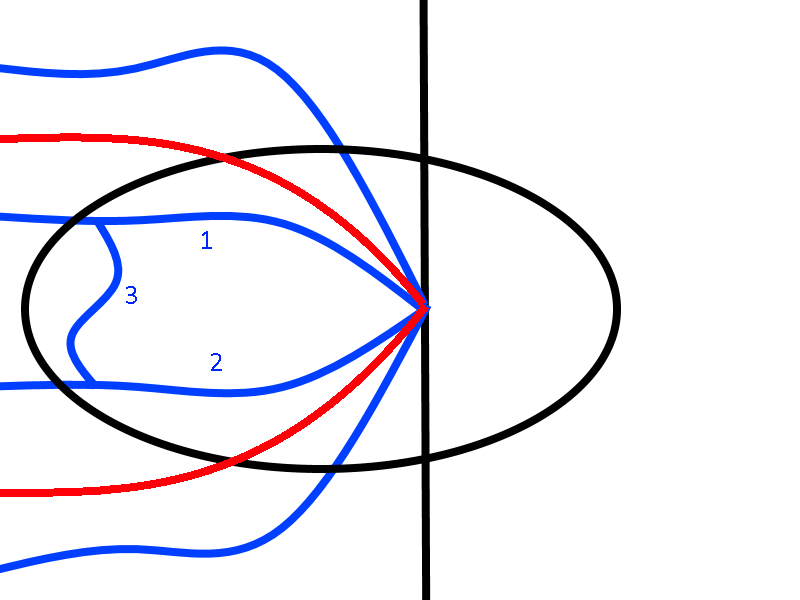
\includegraphics[width=\linewidth]{geodesic_triangle.png}
\end{subfigure}
\begin{subfigure}[b]{0.4\linewidth}
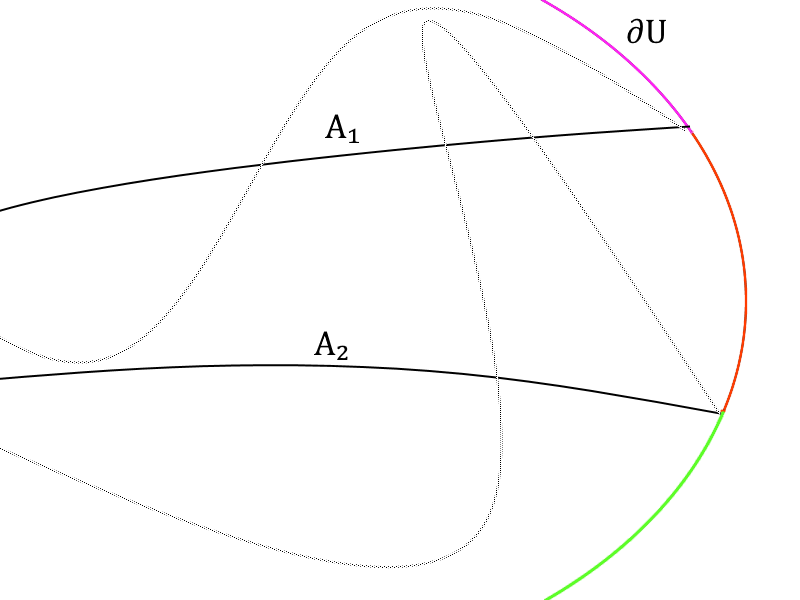
\includegraphics[width=\linewidth]{converse_max.png}
\end{subfigure}
\caption{The left picture illustrates the $d = 2$ case.
The geodesic triangle $T$ is lightly shaded, bounded by the geodesics $\gamma_1, \gamma_2, \overline{QR}$. Here $\{u > y\} = \{v > 0\}$ is shaded, and $\{\tilde v > 0\}$ is darkly shaded.
The right picture illustrates the converse to the maximum principle. The function $u$ is constant on each colored piece of $\partial U$, and its level sets $A_1, A_2$ form a geodesic lamination.
The competitor $v$ has the same trace on $\partial U$, but its level sets (the lighter curves) are not geodesics and so by the coarea formula, $u$ is smaller.}
\label{max_princip_graphs}
\end{figure}

\subsubsection{Minimal lamination implies least gradient}
Now suppose that $\lambda$ is a minimal lamination whose set of leaves is discrete, so every set $A_y$ is minimal and $y$ ranges over a discrete set $\Gamma$.
Fix $U \Subset M$ with Lipschitz boundary, let $T: BV(U) \to L^1(\partial U)$ be the trace map, and let $v$ be a competitor in $U$, thus $v \in BV(U)$ and $Tu = Tv$.
In particular, for every $y \in \Gamma$, $\{Tu \geq y\} = \{Tv \geq y\}$.

By (\ref{convergence of trace}), for any $w \in BV(U)$, $x \in \partial U$, and $z \in \RR$, $T(1_{w > z})(x)$ is the density of $\{w > z\}$ in an infinitesimal neighborhood of $x$.
Let $\varepsilon > 0$ be so small that $\{Tu > y\} = \{Tu > y - 2\varepsilon\}$, which exists since $\Gamma$ is discrete.
If $Tv(x) > y$, then the density of $\{v > y - \varepsilon/2\}$ near $x$ is $1$, so $T(1_{\{v > y - \varepsilon/2\}})(x) = 1$, so 
$$1_{\{Tu > y\}} = 1_{\{Tv > y\}} \leq T(1_{\{v > y - \varepsilon/2\}}).$$
Conversely, if $Tv(x) \leq y - \varepsilon$, then the density of $\{v > y - \varepsilon/2\}$ near $x$ is $0$. Thus 
$$T(1_{\{v > y - \varepsilon/2\}}) \leq T(1_{\{v > y - \varepsilon\}}) \leq 1_{\{Tv > y - \varepsilon\}} = 1_{\{Tu > y - \varepsilon\}} = 1_{\{Tu > y\}}.$$
The inequalities collapse and imply that $1_{\{Tu > y - \varepsilon\}} = T(1_{\{v > y - \varepsilon\}})$.
This is true for $\varepsilon$ arbitrarily small, so
$$1_{\{Tu \geq y\}} = T(1_{\{v \geq y\}}).$$
The left-hand side is $T(1_{\{u > y\}})$ since $u$ is locally constant away from $\lambda$ (since $\Gamma$ is discrete).
Therefore $A_y$ and $1_{\{v \geq y\}}$ are competitors, thus since $A_y$ is minimal, 
\begin{equation}\label{laminationwise least gradient}
|A_y \cap U| \leq |\partial^* \{v \geq y\} \cap U|.
\end{equation}
We now integrate both sides of (\ref{laminationwise least gradient}) against $\dif y$ and apply the coarea formula, Proposition \ref{coarea formula}, to see that
$$\int_U \star |\dif u| = \int_{-\infty}^\infty |A_y \cap U| \dif y \leq \int_{-\infty}^\infty |\partial^* \{v \geq y\} \cap U| \dif y = \int_U \star |\dif v|,$$
    implying that $u$ has least gradient.

\subsection{Radon-Nikod\'ym decomposition}
We finally prove Theorem \ref{Gorny regularity}.
Let $u$ be a function of least gradient on $M$.

Let
\begin{align*}
\hat u(x) &:= \inf\left\{t \in \RR: \lim_{r \to 0} \frac{|\{u \leq t\} \cap B(x, r)|}{|B(x, r)|} = 1\right\},\\
\check u(x) &:= \sup\left\{t \in \RR: \lim_{r \to 0} \frac{|\{u \geq t\} \cap B(x, r)|}{|B(x, r)|} = 1\right\},
\end{align*}
and let $J_u$ be the jumpset of $u$.
Reasoning identically to the proof of \cite[Proposition 3.9]{górny2017planar} we see that $J_u = \{\hat u \neq \check u\}$.
By \cite[Theorem 4.1]{HakkarainenKorteLahtiShanmugalingam+2015}, it follows that $u := \check u$ only has jump discontinuities, and so the minimal lamination $\lambda$ is equal to the jumpset.
Moreover, along each leaf $N \subset M$, the trace of $u$ from each side is constant along $N$, at least after shrinking $M$.
So by Lemma \ref{existence of jump graphs}, there exists a unique (up to additive constants) decomposition $u = u_j - u_c$ such that $u_j$ is locally constant on $M \setminus \lambda$, $u_j$ has the same jumpset, with the same traces on each leaf, as $u$, and $u_c$ has no jump discontinuties.

We claim that $u_j$ has least gradient, as the proof for $u_c$ is similar.
If not, let $v \in BV_\cpt(M)$ satisfy $\int \star|\dif(u_j+v)| < \int \star|\dif u_j|$.
Since $u_j$ has only jump discontinuities and is otherwise locally constant, and $u_c$ has no jump discontinuities, $\dif u_j,\dif u_c$ are mutually singular, thus
\begin{align*}
\int_M \star |\dif u| &\leq \int_M \star |\dif(u+v)| \leq \int_M \star|\dif u_c| + \int_M \star|\dif(u_j + v)| \\
&< \int_M \star |\dif u_c| + \int_M \star |\dif u_j| = \int_M \star |\dif u|,
\end{align*}
a contradiction.
It follows that $u_c$ has least gradient.
Repeating the reasoning from the start of this proof and using the fact that $u_c$ has no jump discontinuities, it follows that $u_c$ is continuous.



\printbibliography

\end{document}
